%%%%%%%%%%%%%%%%%%%%%%%%%%%%%%%%%%%%%%%%%%%%%%%%%%%
%% LaTeX book template                           %%
%% Author:  Amber Jain (http://amberj.devio.us/) %%
%% License: ISC license                          %%
%%%%%%%%%%%%%%%%%%%%%%%%%%%%%%%%%%%%%%%%%%%%%%%%%%%

\documentclass[12pt]{report}
\usepackage[letterpaper, total={6in, 8in}]{geometry}
\usepackage[T1]{fontenc}
\usepackage[utf8]{inputenc}
\usepackage{lmodern}
\usepackage{tikz}
\usetikzlibrary{fadings}
\usetikzlibrary{patterns}
\usetikzlibrary{shadows.blur}
\usetikzlibrary{shapes}
\usepackage{indentfirst}
\usepackage{physics}
\usepackage{mathdots}
\usepackage{extarrows}
\usepackage{setspace}
\usepackage{matlab-prettifier}
\usepackage{csquotes}
\usepackage{biblatex}
\addbibresource{references.bib}
\usepackage{float}


%% GLOSSARY:
\usepackage{glossaries}
\makeglossaries

\newglossaryentry{Angle of Attack}
{
    name=\textit{Angle of Attack},
    description={The angle of offset of the freestream velocity with the $\hat{X}$/$\hat{b}_1$, or longitudinal axis, of the vehicle. This is often denoted with the Greek letter $\alpha$}
}

\newglossaryentry{DoF}
{
    name=\textit{Degree of Freedom},
    description={A free direction of movement for a vehicle. These can be translational or rotational directions}
}

\newacronym{dof}{DoF}{Degree of Freedom}
\newacronym{rhr}{RHR}{Right Hand Rule}

%%%%%%%%%%%%%%%%%%%%%%%%%%%%%%%%%%%%%%%%%%%%%%%%%%%%%%%%%
% Source: http://en.wikibooks.org/wiki/LaTeX/Hyperlinks %
%%%%%%%%%%%%%%%%%%%%%%%%%%%%%%%%%%%%%%%%%%%%%%%%%%%%%%%%%
\usepackage{hyperref}
\usepackage{graphicx}
\usepackage[english]{babel}
\usepackage{fancyhdr}
\usepackage{mathtools}
\mathtoolsset{showonlyrefs} 


%%%%%%%%%%%%%%%%%%%%%%%%%%%%%%%%%%%%%%%%%%%%%%%%%%%%%%%%%%%%%%%%%%%%%%%%%%%%%%%%
% 'dedication' environment: To add a dedication paragraph at the start of book %
% Source: http://www.tug.org/pipermail/texhax/2010-June/015184.html            %
%%%%%%%%%%%%%%%%%%%%%%%%%%%%%%%%%%%%%%%%%%%%%%%%%%%%%%%%%%%%%%%%%%%%%%%%%%%%%%%%

\newenvironment{dedication}
{
   \cleardoublepage
   \thispagestyle{empty}
   \vspace*{\stretch{1}}
   \hfill\begin{minipage}[t]{0.66\textwidth}
   \raggedright
}
{
   \end{minipage}
   \vspace*{\stretch{3}}
   \clearpage
}

%% CODE STUFF
\usepackage{listings}
\usepackage{xcolor}

\definecolor{codegreen}{rgb}{0,0.6,0}
\definecolor{codegray}{rgb}{0.5,0.5,0.5}
\definecolor{codepurple}{rgb}{0.58,0,0.82}
\definecolor{backcolour}{rgb}{0.95,0.95,0.95}

\lstdefinestyle{mystyle}{
    backgroundcolor=\color{backcolour},   
    commentstyle=\color{codegreen},
    keywordstyle=\color{magenta},
    numberstyle=\tiny\color{codegray},
    stringstyle=\color{codepurple},
    basicstyle=\ttfamily\footnotesize,
    breakatwhitespace=false,         
    breaklines=true,                 
    captionpos=t,                    
    keepspaces=true,                 
    numbers=left,                    
    numbersep=5pt,                  
    showspaces=false,                
    showstringspaces=false,
    showtabs=false,                  
    tabsize=4
}



\lstMakeShortInline[style=Matlab-editor]"

\mlttfamily

\setlength{\parskip}{12pt}

\setlength{\headheight}{15pt}

%%%%%%%%%%%%%%%%%%%%%%%%%%%%%%%%%%%%%%%%%%%%%%%%
% Chapter quote at the start of chapter        %
% Source: http://tex.stackexchange.com/a/53380 %
%%%%%%%%%%%%%%%%%%%%%%%%%%%%%%%%%%%%%%%%%%%%%%%%
\makeatletter
\renewcommand{\@chapapp}{}% Not necessary...
\newenvironment{chapquote}[2][2em]
  {\setlength{\@tempdima}{#1}%
   \def\chapquote@author{#2}%
   \parshape 1 \@tempdima \dimexpr\textwidth-2\@tempdima\relax%
   \itshape}
  {\par\normalfont\hfill--\ \chapquote@author\hspace*{\@tempdima}\par\bigskip}
\makeatother

%%%%%%%%%%%%%%%%%%%%%%%%%%%%%%%%%%%%%%%%%%%%%%%%%%%
% First page of book which contains 'stuff' like: %
%  - Book title, subtitle                         %
%  - Book author name                             %
%%%%%%%%%%%%%%%%%%%%%%%%%%%%%%%%%%%%%%%%%%%%%%%%%%%

% Book's title and subtitle
\title{\Huge \textbf{Flight Dynamics Bible}  \\ \huge Everything about 6 Degree of Freedom Modeling}

% Author
\author{\textsc{Hudson Reynolds}
\and
\textsc{Preston Wright}
}

\begin{document}

\pagestyle{fancy}
\renewcommand{\chaptermark}[1]{\markboth{#1}{#1}}
\fancyhead[R]{}
\fancyhead[L]{\thechapter\ --\ \leftmark}

%\frontmatter
\maketitle

%%%%%%%%%%%%%%%%%%%%%%%%%%%%%%%%%%%%%%%%%%%%%%%%%%%%%%%%%%%%%%%
% Add a dedication paragraph to dedicate your book to someone %
%%%%%%%%%%%%%%%%%%%%%%%%%%%%%%%%%%%%%%%%%%%%%%%%%%%%%%%%%%%%%%%
\begin{dedication}
    This document is dedicated to Purdue Space Program Liquids. PSP Liquids has given us a vast amount of experience and means to explore the realm of Flight Dynamics. We hope that we can contribute to the wealth of information provided by PSP with this document.
\end{dedication}

%%%%%%%%%%%%%%%%%%%%%%%%%%%%%%%%%%%%%%%%%%%%%%%%%%%%%%%%%%%%%%%%%%%%%%%%
% Auto-generated table of contents, list of figures and list of tables %
%%%%%%%%%%%%%%%%%%%%%%%%%%%%%%%%%%%%%%%%%%%%%%%%%%%%%%%%%%%%%%%%%%

\begin{spacing}{.5}
    \tableofcontents
    \listoftables
    \listoffigures
\end{spacing}

%\mainmatter

%%%%%%%%%%%
% Preface %
%%%%%%%%%%%
\chapter*{Preface}
Preston and I began working on the Flight Dynamics sub-team in the fall of 2023. From May 2024 to January 2025, we focused our efforts on creating a 6-DoF model from scratch. During this time, we learned a lot about the mathematics and physics involved in creating such a model. We were often faced with frustration with different conventions and poor explanations of certain topics, all of which were exacerbated by the difficulty of what we were learning. This made much of the material intractable. In this document, we hope to provide detailed explanations of all the necessary concepts in one place to make this journey easier for those who may need it in the future. 

Furthermore, we hope that this document can be used by those outside the realm of flight dynamics to better understand the methodologies and inner workings of a 6-DoF model. Often, we have seen that a 6-DoF model is treated as a ‘black box’, where inputs go in and outputs come out. We hope that this document can provide a level of understanding adequate to allow greater collaboration between those working within and outside of flight dynamics.

In this document, we will be using excerpts of MATLAB script in some examples (code less than a page is included inline, and longer code is in the appendix) but our hope is that our explanations are thorough enough to facilitate the creation of a 6-DoF in any coding language. MATLAB facilitates the use of quite short code because of the number of built-in functions, but we include derivations for most of these equations or sources describing these derivations.

To use this document to its fullest extent, we recommend that you write scripts as you learn and use this document for reference and as a guide as you build or improve your own models.

In this first edition, we cover primarily the translational and rotational dynamics needed to set up a 6-DoF model. We also touch on subjects relating to the implementation of these equations in MATLAB and best practices. These are, in our opinion, the fundamental things that need to be understood before working on other aspects of a flight dynamics model. As such, these subjects comprise a large majority of both the effort and the length of the first edition.

Some other areas are also covered in this document but are not fully explained because Preston and I do not have the experience to give full authority on these subjects. However, as we learn more, this document is growing every day. In future editions, we hope to expand some of these other sections, especially those related to aerodynamics, to better serve those in the future who may hope to recreate the work we have done here.

% \section*{About the companion website}
% The website\footnote{\url{https://github.com/amberj/latex-book-template}} for this file contains:
% \begin{itemize}
%   \item A link to (freely downlodable) latest version of this document.
%   \item Link to download LaTeX source for this document.
%   \item Miscellaneous material (e.g. suggested readings etc).
% \end{itemize}

%%%%%%%%%%%%%%%%%%%%%%%%%%%%%%%%%%%%
% Give credit where credit is due. %
% Say thanks!                      %
%%%%%%%%%%%%%%%%%%%%%%%%%%%%%%%%%%%%
\section*{Acknowledgments}
\begin{itemize}
\item We would like give special thanks to Prof. Cunningham and Prof. Frueh for their help in reviewing our 6-DoF Model. Professor Frueh's notes have been especially helpful in compiling the information present in this document.

\end{itemize}

\chapter{Overview}

\begin{chapquote}{Carl Sagan}
''If you wish to make an apple pie from scratch, you must first invent the universe.''
\end{chapquote}

In much the same way, we must construct all of the mathematical background required to make a 6-DoF from the ground up. This chapter details the general requirements and an outline of the process we will be following.

\section{Necessary Background}
The goal of this document is to provide a comprehensive overview of the process and means of creating, maintaining, and building on a 6 Degree of Freedom model. Although we strive to make the document as easy as possible to understand, there are some instances where technical jargon is necessary and a strong understanding of mathematical concepts is required. 

Any time important technical jargon is required, we will \textit{italicize} the word for recognition. It is important to learn these terms to effectively and concisely describe your work. That being said, we attempt to keep the usage of jargon to a minimum. Because we italicize words in this manner, we choose to additionally underline any book titles present in the text. A glossary with these terms has also been added so that all of these words are included in a single location. 

To aid in comprehensibility, we have added sources that we find especially useful and avoided the use of superfluous sources. These sources are hyperlinked for ease of access. In addition, useful links and footnotes have been highlighted in red boxes to be easily located. 

To fully comprehend and successfully use this document, it is recommended that you have a good understanding of calculus, linear algebra, and calculus-based physics. A rudimentary understanding of differential equations and dynamics will also prove useful but is not strictly required.

Some concepts will arise in this document that are derived from graduate-level coursework and complex mathematics. In these instances, we may not attempt to derive the background and full understanding, but rather only what is necessary for building a 6-DoF model. In these cases, we also try to link to source material if you are inclined to learn more about those topics.

\section{Why 6-DoF?}
Let’s start off with some terminology in this section. A \gls{dof} refers to the number of ways an object can move in space. A more technically precise and rigorous definition defines this as the number of independent parameters that define the state. It is common to see 1-DoF, 3-DoF, and 6-DoF models all used in aerospace applications. Each of these are useful constructs, and often a simulation with more degrees of freedom is not necessarily better, depending on the scenario.
\subsection{1-DoF}
The first modeling that is often done for the sizing of rockets may use 1-DoF modeling. In this type of model, there is only one axis along which an object may translate or rotate about. In this case of rocket modeling, the only degree of freedom is the vertical height of the rocket. The goal of this type of model is mainly to provide a heuristic for determining rocket performance in the very preliminary stages of sizing by estimating the maximum altitude they can achieve.

Another example of this type of model is a simple mass-spring system along one axis. Such models may be useful for estimating the vibrations of bodies or as a first order approximation of fuel slosh.

We will use the example of a 1-DoF in section 2.1 to explain the creation of equations of motion in the simplest way. However, these models are often too constrained to give the most valuable information about a system, which is why 3-DoF and 6-DoF models are more often used.
\subsection{3-DoF}
After 1-DoF, the next step up is often a 3-DoF model. This type of model should be familiar to all flight dynamics members, as it is the subject of our onboarding project. In a 3-DoF model, there may be any combination of translational degrees of freedom and rotational degrees of freedom.

Often, 3-DoF modelling is utilized when either the rotational dynamics or translational dynamics of an object are considered unimportant. One example of this may be the calculation of an interplanetary transfer. The primary concern of the simulation is not the orientation of the satellite, but rather the location and velocity of the satellite at various points in 3D space. 

Another example of this type of model is planar motion. Often, problems in engineering are constrained in some way. Very often, we can consider one of the translational degrees of freedom to be non-important to the problem. This simplification allows us to greatly reduce the scope of the problem. One consequence of this action is that rotations are only permitted in a single axis. With two translational and one rotational degree of freedom, we can create useful models of many systems without great complexity.

Although the rest of this document will discuss 6-DoF models, really consider if you need that full complexity for your model! Often, a 3-DoF model is perfectly adequate for a large variety of problems without the hassle incurred by a 6-DoF model. 
\subsection{6-DoF}
6-DoF models are the most complex representation of a mechanical system. In 3D-space, there are only 6 possible degrees of freedom, and we simulate the dynamics in all of them.

Doing so is quite a difficult challenge, but it is not insurmountable. With careful planning, it is possible to gain an appreciation and understanding of the dynamics of a full 3D system. Doing so allows unrivaled modeling potential. In the case of a rocket, the primary reason that modeling in 6-DoF is so important is because it allows us to analyze the aerodynamic stability of the system. In both 1-DoF and 3-DoF modeling, this important aspect of the system is largely neglected.
\subsection{Structure Hierarchy of a 6-DoF}
An ideal 6-DoF not only models the motion of a vehicle through the atmosphere as accurately as possible but is also well-structured and easily readable. Strict adherence to an agreed upon and appropriate set of coding standards is essential for a successful program. These cover everything from naming conventions to heading structure, and make the integration of codes from multiple contributors more seamless.

Within the structure of a 6-DoF, there are three main, large “blocks” of code that are executed in sequence. The first is the initialization section. This is where all known, fixed parameters of the vehicle, atmosphere, and physics are initialized to be called later in the program. The second section is the integrator. This block utilizes a certain integration scheme to step through time, calculating the derivatives of the vehicle’s \textit{state vector}. Within the integrator, there are two major sub-blocks corresponding to two sets of dynamics: the forces and the moments. The forces section takes on the more familiar Newtonian Dynamics – regarding Position, Velocity, and Acceleration - that are seen in a high school physics class. The moments section takes on the Attitude Dynamics – orientation in space - of the vehicle. This can take the form of either Euler Angles or Parameters, which will be discussed further later. The final block is the visualizer block. This section writes pertinent information to matrices, animates the movement of the vehicle from launch to land, and outputs graphs of important metrics for the user to visualize.

Each of the previously mentioned sections will be discussed in more detail throughout this document.

\chapter{Newtonian Dynamics}\label{sec: Newtonian Dynamics}
\begin{chapquote}{Isaac Newton}
''I can calculate the motion of heavenly bodies, but not the madness of people.''
\end{chapquote}
The first step when approaching any physics problem of this type is to consider the Newtonian dynamics of the system. In our case, we define Newtonian dynamics as the translational dynamics of the system as well as the moments acting on the system. This differs from particle dynamics because we are considering a rigid body which can exhibit rotation. The exploration of this rotation will be explored in much more detail in Section \ref{sec:attitude dynamics}. 
\section{The 1-DoF Case:}\label{sec: The 1DoF Case}
To begin our exploration of Newtonian dynamics, we will return to the example of the 1-DoF which we used earlier. Our goal with this is to use a simple example you are familiar with from high school physics and bring it up to speed with the terminology and techniques we will use for more complex analysis.

In Figure 1 below, we show an example of a very simple 1-DoF system free body diagram. We will use this example to explain the process of calculating the Newtonian dynamics in 1-dimension, which we then expand to the full 3D case. 

\tikzset{every picture/.style={line width=0.75pt}} %set default line width to 0.75pt        

\begin{figure}[ht]
    \centering
    %\includegraphics[width=0.5\linewidth]{}
    
    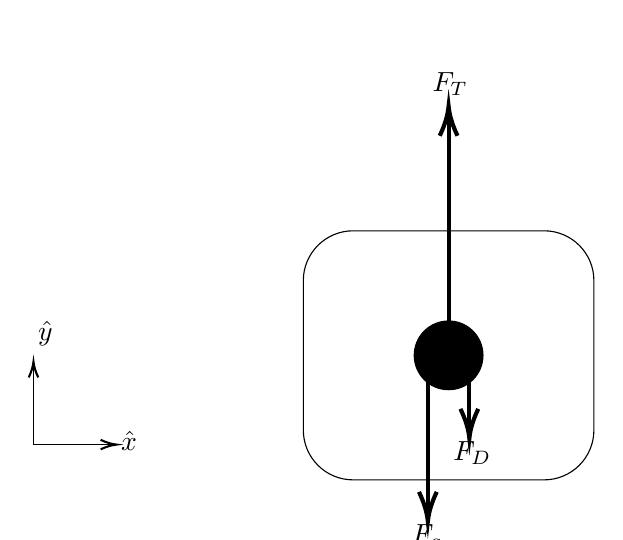
\begin{tikzpicture}[x=0.75pt,y=0.75pt,yscale=-1,xscale=1]
%uncomment if require: \path (0,308); %set diagram left start at 0, and has height of 308

%Rounded Rect [id:dp5842362308374554] 
\draw  [color={rgb, 255:red, 0; green, 0; blue, 0 }  ,draw opacity=1 ][fill={rgb, 255:red, 255; green, 255; blue, 255 }  ,fill opacity=1 ] (260,144) .. controls (260,130.75) and (270.75,120) .. (284,120) -- (376,120) .. controls (389.25,120) and (400,130.75) .. (400,144) -- (400,216) .. controls (400,229.25) and (389.25,240) .. (376,240) -- (284,240) .. controls (270.75,240) and (260,229.25) .. (260,216) -- cycle ;
%Straight Lines [id:da22630541270037763] 
\draw [line width=1.5]    (330,180) -- (330,63) ;
\draw [shift={(330,60)}, rotate = 90] [color={rgb, 255:red, 0; green, 0; blue, 0 }  ][line width=1.5]    (14.21,-4.28) .. controls (9.04,-1.82) and (4.3,-0.39) .. (0,0) .. controls (4.3,0.39) and (9.04,1.82) .. (14.21,4.28)   ;
%Straight Lines [id:da4912651471508729] 
\draw [line width=1.5]    (340,180) -- (340,217) ;
\draw [shift={(340,220)}, rotate = 270] [color={rgb, 255:red, 0; green, 0; blue, 0 }  ][line width=1.5]    (14.21,-4.28) .. controls (9.04,-1.82) and (4.3,-0.39) .. (0,0) .. controls (4.3,0.39) and (9.04,1.82) .. (14.21,4.28)   ;
%Shape: Circle [id:dp11471774870022611] 
\draw  [fill={rgb, 255:red, 0; green, 0; blue, 0 }  ,fill opacity=1 ] (313.44,180) .. controls (313.44,170.85) and (320.85,163.44) .. (330,163.44) .. controls (339.15,163.44) and (346.56,170.85) .. (346.56,180) .. controls (346.56,189.15) and (339.15,196.56) .. (330,196.56) .. controls (320.85,196.56) and (313.44,189.15) .. (313.44,180) -- cycle ;
%Straight Lines [id:da07105152032768414] 
\draw    (130,223) -- (130,185) ;
\draw [shift={(130,183)}, rotate = 90] [color={rgb, 255:red, 0; green, 0; blue, 0 }  ][line width=0.75]    (7.65,-2.3) .. controls (4.86,-0.97) and (2.31,-0.21) .. (0,0) .. controls (2.31,0.21) and (4.86,0.98) .. (7.65,2.3)   ;
%Straight Lines [id:da477096952774564] 
\draw    (130,223) -- (168,223) ;
\draw [shift={(170,223)}, rotate = 180] [color={rgb, 255:red, 0; green, 0; blue, 0 }  ][line width=0.75]    (7.65,-2.3) .. controls (4.86,-0.97) and (2.31,-0.21) .. (0,0) .. controls (2.31,0.21) and (4.86,0.98) .. (7.65,2.3)   ;
%Straight Lines [id:da5415789935745218] 
\draw [line width=1.5]    (320,180) -- (320,257) ;
\draw [shift={(320,260)}, rotate = 270] [color={rgb, 255:red, 0; green, 0; blue, 0 }  ][line width=1.5]    (14.21,-4.28) .. controls (9.04,-1.82) and (4.3,-0.39) .. (0,0) .. controls (4.3,0.39) and (9.04,1.82) .. (14.21,4.28)   ;

% Text Node
\draw (331,220.4) node [anchor=north west][inner sep=0.75pt]    {$F_{D}$};
% Text Node
\draw (321,42.4) node [anchor=north west][inner sep=0.75pt]    {$F_{T}$};
% Text Node
\draw (171,215.4) node [anchor=north west][inner sep=0.75pt]    {$\hat{x}$};
% Text Node
\draw (131,162.4) node [anchor=north west][inner sep=0.75pt]    {$\hat{y}$};
% Text Node
\draw (311,260.4) node [anchor=north west][inner sep=0.75pt]    {$F_{g}$};


\end{tikzpicture}
    \caption{1-DoF Forces on a body}
    \label{Figure 1}
\end{figure}

In Figure \ref{Figure 1}, a total of three forces are shown, all of which act along the  direction. The colinearity of all these forces is what makes this a 1-DoF model. The three forces shown are the thrust force, the drag force, and the gravity force.

Following what you may do in an introductory physics class, we will describe each of these forces via their functional form. These are described in Table \ref{Force Equations 1 DoF}. 

\begin{table}
\centering
\caption{Functional Form of Force Equations}
\label{Force Equations 1 DoF}
\begin{tabular}{l | l}
Force & Functional Form \\
\hline
 $F_g$&  $-mg$\\
 $F_D$&  $-\frac{1}{2} \rho_{\infty} V^2_{\infty}SC_D$\\
 $F_T$&  $F_T\cdot[1-u(t-t_b)], t\le0$\\

\end{tabular}

\end{table}
The notation here is important to understand. In future AAE classes at Purdue, this is likely the notation that you will see. Terms with the subscript $\infty$ denote \textit{freestream} quantities, those that are freely flowing far away from the body of interest. Also of note is the unit step function, which is a function which has value zero until reaching time $t_b$, where it thereafter equals one. The quantity  $\rho$ refers to the density of the fluid, and $S$ to the \textit{reference area}. The \textit{drag coefficient} is $C_D$, a term which encapsulates the very complex nature of the fluid flow around an object. Calculating the value of  will be explored more deeply in later sections of this document. For now, we may assume a constant value.

It is helpful to think about these quantities as vectors, because we can add them together to achieve a resultant.\footnote{More formally, we define this as a linear space, where multiplicative and additive properties are preserved. This formal definition allows us to apply this to any arbitrarily number of dimensions. } In the 1-dimensional case this is quite trivial since all vectors along the $\hat{y}$ unit vector, but this will become increasingly important as we move to higher dimensions.
\subsection{Numerical Integration in the 1-DoF}\label{sec: Numerical Integration in the 1DoF}
Now we will move into something that you may have not seen before. Given all the forces, we normally apply Newton’s 2\textsuperscript{nd} Law, $\sum{\vec{F}}=m\vec{a}$ , to arrive at an expression for the acceleration as shown in \eqref{eq2}. Doing so might look something like this:
\begin{gather}
F_T \cdot [1-u(t-t_b)]-\frac{1}{2}\rho_{\infty}V_{\infty}^2SC_D-mg=m\vec{a}\label{eq1} \\
\vec{a}=\frac{F_T \cdot [1-u(t-t_b)]-\frac{1}{2}\rho_{\infty}V_{\infty}^2SC_D}{m}-g\label{eq2}
\end{gather}
 From here, we use integration to find the velocity and then position of the object with time. Formally, we might define this formally as:
 $$\vec{V}=\int{\vec{a}}{dt}$$
However, you may notice something strange with our equation. In our expression for acceleration, we need to know the velocity. However, we do not know the velocity without integrating the equation first. This puts us in a chicken v. egg situation, so we must take a different approach to the problem. \footnote{Sometimes systems like this can be solved with traditional ODE methods. However, most complex systems like our 6-DoF have no known analytical solutions. We will focus on numerical integration because it will be more useful in general. }

The way we resolve this is to make an approximation of the solution in a process called \textit{Numerical Integration. }Here, we will outline the simplest type of numerical integration, known as Euler’s Method. This section aims to show how to implement Euler’s method in code, and the mathematical reasoning will be given a more formal treatment in section 5. We will describe more complex numerical integration schemes and why you might want to use them, but it’s good to see the code for a simple case first.

Euler’s Method involves discretizing our time interval. You may remember the concept of a Riemann Sum from calculus, where you approximate an integral in discrete time steps. We will take a similar approach with Euler’s Method. Euler’s method is applicable to solving first order ordinary differential equations (ODE’s). However, in our problem, we have a second order differential equation, because $\vec{a}=\ddot{y}$.

To resolve this issue, we will make this one differential equation into a system of first order differential equations. In general, we can convert an nth-order ODE into a system of n first-order ODEs.

In this case, we define a variable, . Now, we can express equation \eqref{eq2} as a system of two differential equations:

\begin{gather}\label{system}
        \dot{v}=\frac{F_T \cdot [1-u(t-t_b)]-\frac{1}{2}\rho_{\infty}V_{\infty}^2SC_D}{m}-g\\
    \dot{y}=v
\end{gather}

Now, we will apply Euler’s method to solve the problem. We will use the following steps to do so, using equation \eqref{system}as our example:

1. Rewrite the system in Leibniz notation, where $\dot{x}=\frac{dx}{dt}$.

2. Perform separation of variables, to arrive at $dx=v\cdot dt$.

3. Discretize the equation by ‘converting’  $dx$ and $dt$ to $\Delta x$ and $\Delta t$.\footnote{Note that we are not ‘converting’ in the sense of an equality, since the equations are no longer equivalent when we convert a differential element into a discrete one. We are just making an approximation of the true solution. Luckily, numerical integration schemes can get us quite close to true solutions. }

4. Rewrite $\Delta x$ as $x_{new}-x_{old}$. We can rearrange the equation as $x_{new}=v\cdot \Delta t + x_{old}$

5. To start, we define an initial state. This initial state will be the first value of $x_{old}$. 

6. Iterate through values of $\Delta t$ until the desired time of simulation is achieved.

We follow the same process for the integration of acceleration to find the velocity. Of note, we will use the previous value of $v$ in the computation of the new acceleration. Note that a more formal definition of Euler’s method is given in section 5.1.

We also show this example in MATLAB Script \ref{Script 1} below. Note that $\frac{1}{2}\rho_{\infty}SC_D$ is called $k$ in the script for simplicity. This simplification assumes that $\rho_{\infty}$ and the $C_D$ are constant, which we will later see is a quite poor assumption but is okay for a first approximation.

\lstset{style=mystyle}

\lstinputlisting[language=Matlab, caption=1 DoF]{OneDofEuler.m}\label{Script 1}

There are a few important things to note about the MATLAB implementation of the script. Firstly, the only force that is defined outside of the loop is gravity, because the magnitude and direction of this force is independent of the current state of the system. We contrast this with the drag force and the thrust, which must be calculated on every iteration through the algorithm to find an updated value for the force.

We also note the use of the Heaviside function. This is functionally identical to a unit step function, just a different notation.

\section{The 3-DoF Case}\label{sec: 3DoF Case}
\subsection{Vectors in the 3-DoF Case:}
For Newtonian Dynamics, the most complex case is full 3D translational motion. Luckily, nothing very fundamental changes as compared to the 1-DoF case. The most important difference is the use of vector notation for compactness and clarity of mathematics and code. For position ($\vec{r}$), velocity ($\vec {v}$), and acceleration ($\vec{a}$), we represent them as tri-dimensional column vectors:

\begin{gather}
    \vec{r}=\begin{bmatrix}
        x_1\\
        x_2\\
        x_3
    \end{bmatrix},
    \vec{v}=\begin{bmatrix}
        \dot{x}_1\\
        \dot{x}_2\\
        \dot{x}_3\\
    \end{bmatrix},
        \vec{a}=\begin{bmatrix}
        \ddot{x}_1\\
        \ddot{x}_2\\
        \ddot{x}_3\\
    \end{bmatrix}
\end{gather}
This is done not only for the sake of compactness, but also to facilitate the use of matrix operations for translation between reference frames. This concept is further explored in section 3. For this reason, expressing these elements in vectors will become crucial as we move forward. In MATLAB, we express a tri-dimensional column vector as:
\begin{lstlisting}[language=Matlab]
pos=[0;0;0];
\end{lstlisting}
Where each semicolon represents a new row of the vector. We define a row vector by using a comma instead of a semicolon: 
\begin{lstlisting}[language=Matlab]
pos=[0,0,0];
\end{lstlisting}
Often, it is useful to convert between a row and column vector in MATLAB because some functions will expect the input to be in a different format. We can do so with a transposition. In MATLAB, this looks like: 
\begin{lstlisting}
pos=[0,0,0];
\end{lstlisting}
\subsection{Vector directions in the 3-DoF}
We present below a modified version of the 1-DoF below in full 3D in Figure \ref{fig:3 DoF Forces}.


\tikzset{every picture/.style={line width=0.75pt}} %set default line width to 0.75pt        

\begin{figure}[ht]
    \centering
    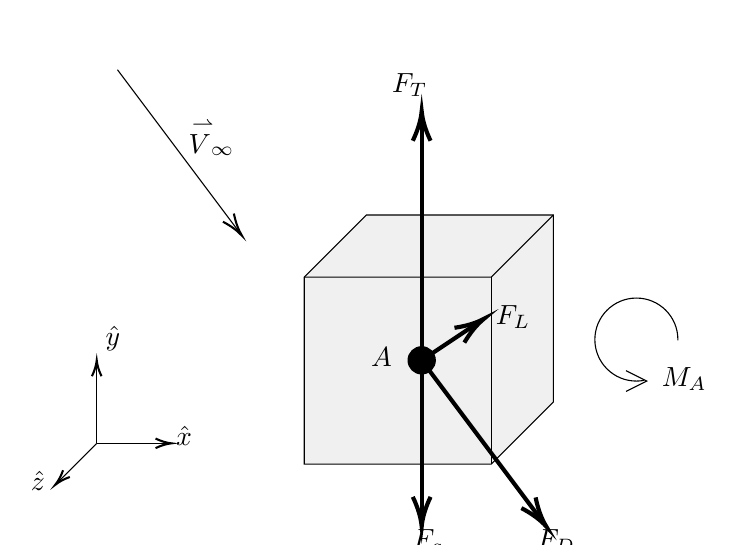
\begin{tikzpicture}[x=0.75pt,y=0.75pt,yscale=-1,xscale=1]
%uncomment if require: \path (0,308); %set diagram left start at 0, and has height of 308

%Shape: Cube [id:dp15885218660825062] 
\draw  [fill={rgb, 255:red, 155; green, 155; blue, 155 }  ,fill opacity=0.15 ] (260,129.92) -- (289.92,100) -- (380,100) -- (380,190.08) -- (350.08,220) -- (260,220) -- cycle ; \draw   (380,100) -- (350.08,129.92) -- (260,129.92) ; \draw   (350.08,129.92) -- (350.08,220) ;
%Straight Lines [id:da7537274804871096] 
\draw    (160,210) -- (160,172) ;
\draw [shift={(160,170)}, rotate = 90] [color={rgb, 255:red, 0; green, 0; blue, 0 }  ][line width=0.75]    (7.65,-2.3) .. controls (4.86,-0.97) and (2.31,-0.21) .. (0,0) .. controls (2.31,0.21) and (4.86,0.98) .. (7.65,2.3)   ;
%Straight Lines [id:da28051238395124845] 
\draw    (160,210) -- (194,210) ;
\draw [shift={(196,210)}, rotate = 180] [color={rgb, 255:red, 0; green, 0; blue, 0 }  ][line width=0.75]    (7.65,-2.3) .. controls (4.86,-0.97) and (2.31,-0.21) .. (0,0) .. controls (2.31,0.21) and (4.86,0.98) .. (7.65,2.3)   ;
%Straight Lines [id:da0491508391303197] 
\draw    (160,210) -- (141.41,228.59) ;
\draw [shift={(140,230)}, rotate = 315] [color={rgb, 255:red, 0; green, 0; blue, 0 }  ][line width=0.75]    (7.65,-2.3) .. controls (4.86,-0.97) and (2.31,-0.21) .. (0,0) .. controls (2.31,0.21) and (4.86,0.98) .. (7.65,2.3)   ;
%Straight Lines [id:da4424478744689285] 
\draw    (170,30) -- (228.8,108.4) ;
\draw [shift={(230,110)}, rotate = 233.13] [color={rgb, 255:red, 0; green, 0; blue, 0 }  ][line width=0.75]    (10.93,-3.29) .. controls (6.95,-1.4) and (3.31,-0.3) .. (0,0) .. controls (3.31,0.3) and (6.95,1.4) .. (10.93,3.29)   ;
%Straight Lines [id:da9341165159771404] 
\draw [line width=1.5]    (316.56,170) -- (316.56,247) ;
\draw [shift={(316.56,250)}, rotate = 270] [color={rgb, 255:red, 0; green, 0; blue, 0 }  ][line width=1.5]    (14.21,-4.28) .. controls (9.04,-1.82) and (4.3,-0.39) .. (0,0) .. controls (4.3,0.39) and (9.04,1.82) .. (14.21,4.28)   ;
%Straight Lines [id:da4700324062294746] 
\draw [line width=1.5]    (316.56,170) -- (374.76,247.6) ;
\draw [shift={(376.56,250)}, rotate = 233.13] [color={rgb, 255:red, 0; green, 0; blue, 0 }  ][line width=1.5]    (14.21,-4.28) .. controls (9.04,-1.82) and (4.3,-0.39) .. (0,0) .. controls (4.3,0.39) and (9.04,1.82) .. (14.21,4.28)   ;
%Straight Lines [id:da6206056974950449] 
\draw [line width=1.5]    (316.56,170) -- (316.56,53) ;
\draw [shift={(316.56,50)}, rotate = 90] [color={rgb, 255:red, 0; green, 0; blue, 0 }  ][line width=1.5]    (14.21,-4.28) .. controls (9.04,-1.82) and (4.3,-0.39) .. (0,0) .. controls (4.3,0.39) and (9.04,1.82) .. (14.21,4.28)   ;
%Shape: Circle [id:dp9278618893074794] 
\draw  [fill={rgb, 255:red, 0; green, 0; blue, 0 }  ,fill opacity=1 ] (310,170) .. controls (310,166.38) and (312.94,163.44) .. (316.56,163.44) .. controls (320.19,163.44) and (323.13,166.38) .. (323.13,170) .. controls (323.13,173.62) and (320.19,176.56) .. (316.56,176.56) .. controls (312.94,176.56) and (310,173.62) .. (310,170) -- cycle ;
%Straight Lines [id:da05847350311292765] 
\draw [line width=1.5]    (316.56,170) -- (344.07,151.66) ;
\draw [shift={(346.56,150)}, rotate = 146.31] [color={rgb, 255:red, 0; green, 0; blue, 0 }  ][line width=1.5]    (14.21,-4.28) .. controls (9.04,-1.82) and (4.3,-0.39) .. (0,0) .. controls (4.3,0.39) and (9.04,1.82) .. (14.21,4.28)   ;
%Shape: Arc [id:dp5580370574812169] 
\draw  [draw opacity=0] (423.67,179.66) .. controls (422.48,179.88) and (421.25,180) .. (420,180) .. controls (408.95,180) and (400,171.05) .. (400,160) .. controls (400,148.95) and (408.95,140) .. (420,140) .. controls (431.05,140) and (440,148.95) .. (440,160) .. controls (440,160.15) and (440,160.29) .. (440,160.44) -- (420,160) -- cycle ; \draw   (423.67,179.66) .. controls (422.48,179.88) and (421.25,180) .. (420,180) .. controls (408.95,180) and (400,171.05) .. (400,160) .. controls (400,148.95) and (408.95,140) .. (420,140) .. controls (431.05,140) and (440,148.95) .. (440,160) .. controls (440,160.15) and (440,160.29) .. (440,160.44) ;  
\draw   (415,175) -- (425,180) -- (415,185) ;

% Text Node
\draw (197,200.4) node [anchor=north west][inner sep=0.75pt]    {$\hat{x}$};
% Text Node
\draw (163,152.4) node [anchor=north west][inner sep=0.75pt]    {$\hat{y}$};
% Text Node
\draw (127,222.4) node [anchor=north west][inner sep=0.75pt]    {$\hat{z}$};
% Text Node
\draw (203,52.4) node [anchor=north west][inner sep=0.75pt]    {$\stackrel {\rightharpoonup}{V}_{\infty }$};
% Text Node
\draw (311,250.4) node [anchor=north west][inner sep=0.75pt]    {$F_{g}$};
% Text Node
\draw (371,250.4) node [anchor=north west][inner sep=0.75pt]    {$F_{D}$};
% Text Node
\draw (301,30.4) node [anchor=north west][inner sep=0.75pt]    {$F_{T}$};
% Text Node
\draw (351,142.4) node [anchor=north west][inner sep=0.75pt]    {$F_{L}$};
% Text Node
\draw (431,172.4) node [anchor=north west][inner sep=0.75pt]    {$M_{A}$};
% Text Node
\draw (291,162.4) node [anchor=north west][inner sep=0.75pt]    {$A$};


\end{tikzpicture}

    \caption{3-DoF Forces on a Body}
    \label{fig:3 DoF Forces}
\end{figure}

As compared to 1-DoF case, we have three new quantities that are present. The first of these is $\vec{V}_{\infty}$, the freestream airflow vector, being shown on the diagram.\footnote{Freestream velocity  is drawn in the direction of incoming air by convention. However, for calculations, we will use the convention that  is the direction of the velocity of the vehicle (opposite sign to drawing).} This is represented diagrammatically because it no longer must be along the $\hat{y}$ direction. When we have an angle between the nose (the direction through which the thrust force points in Figure 2) and the freestream velocity, we refer to this as an \gls{Angle of Attack}. This angle of attack is often denoted with the letter $\alpha$. We will discuss angle of attack and its effects more in section 4. For now, we simply need to understand how to calculate  given the vector through the nose and the freestream velocity vector.

To do this, we use the fact that the dot product is related to the cosine of the angle between the vectors. Denoting the vector through the nose of the rocket , we can find the angle of attack as:
\begin{equation}\label{eq:alpha}
    \alpha=cos^{-1}\left(\frac{\hat{X}\cdot \vec{V}_{\infty}}{||\hat{X}||\ ||\vec{V}_{\infty}||}\right)
\end{equation}

The next new quantity is $F_L$, the force of lift. The force of lift is always perpendicular in direction to $\vec{V}_{\infty}$. Knowing this, we can find the direction of the force of lift as:
\begin{equation}\label{eq:Lift}
    \hat{L}=\frac{(\hat{V}_{\infty} \times \hat{X}) \times \hat{V}_{\infty}}{||(\hat{V}_{\infty} \times \hat{X}) \times \hat{V}_{\infty}||}
\end{equation}
Here, the cross product is used because it generates a vector orthogonal to the two input vectors. This is exactly the property that we need when defining lift.

For the sake of completeness, we should also note that the force of drag lies opposite the direction of . This is much simpler to calculate, and looks like:
$$\hat{D}=\frac{-\hat{V}_{\infty}}{||\hat{V}_{\infty}||}$$

The last force directions to define are the direction of thrust and the direction of gravity. Luckily, these are easily defined because they point directly along basis vectors.\footnote{We assume here that there is no misalignment in the thrust vector and it is coincident with the  vector.} The force of gravity is defined with respect to the inertial reference frame and is defined in \eqref{eq:Fg}. The force of thrust is defined with respect to the vector pointing through the nose, $\hat{X}$, and is shown in \eqref{eq:Ft}:
\begin{equation}\label{eq:Fg}
    \vec{F}_g=-mg\cdot \hat{y}
\end{equation}
\begin{equation}\label{eq:Ft}
    \vec{F}_T=F_T\cdot \hat{X}
\end{equation}
\subsection{Moments}\label{sec:moments}
The last new quantity is the moment about point A, denoted $M_A$. For now, we will simply note that for an arbitrary selection of point A, we will have a rotational moment that is generated because the forces on the body do not necessarily act through point A, even if it is the center of mass (see section 4 for more details). In Figure\ref{fig:3 DoF Forces}, we have drawn all of the forces acting through a single point for simplicity, but this is not generally the case.

For our rocket modeling, it is generally assumed that gravity and thrust act about the center of gravity, and the aerodynamic forces about the center of pressure (more on this in 4.1.1).

We will show how to compute this moment if the location of the center of gravity and the center of pressure is known. To show this, we will briefly return the 2D case for illustration, but keep in mind that this concept is extensible in 3D. We show this in Figure \ref{fig:Moments}.

\begin{figure}
    \centering
    
\tikzset{every picture/.style={line width=0.75pt}} %set default line width to 0.75pt        

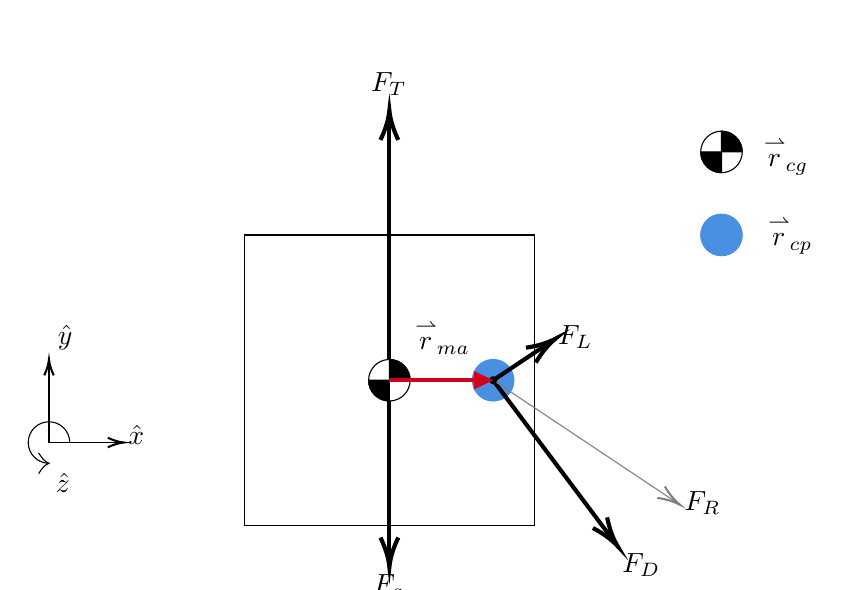
\begin{tikzpicture}[x=0.75pt,y=0.75pt,yscale=-1,xscale=1]
%uncomment if require: \path (0,300); %set diagram left start at 0, and has height of 300

%Shape: Rectangle [id:dp16059631350753278] 
\draw   (224,90) -- (364,90) -- (364,230) -- (224,230) -- cycle ;
%Shape: Circle [id:dp26152316559967836] 
\draw   (284,160) .. controls (284,154.48) and (288.48,150) .. (294,150) .. controls (299.52,150) and (304,154.48) .. (304,160) .. controls (304,165.52) and (299.52,170) .. (294,170) .. controls (288.48,170) and (284,165.52) .. (284,160) -- cycle ;
%Straight Lines [id:da4396178512453982] 
\draw [line width=1.5]    (294,150) -- (294,33) ;
\draw [shift={(294,30)}, rotate = 90] [color={rgb, 255:red, 0; green, 0; blue, 0 }  ][line width=1.5]    (14.21,-4.28) .. controls (9.04,-1.82) and (4.3,-0.39) .. (0,0) .. controls (4.3,0.39) and (9.04,1.82) .. (14.21,4.28)   ;
%Straight Lines [id:da6367078669315451] 
\draw [line width=1.5]    (294,170) -- (294,247) ;
\draw [shift={(294,250)}, rotate = 270] [color={rgb, 255:red, 0; green, 0; blue, 0 }  ][line width=1.5]    (14.21,-4.28) .. controls (9.04,-1.82) and (4.3,-0.39) .. (0,0) .. controls (4.3,0.39) and (9.04,1.82) .. (14.21,4.28)   ;
%Shape: Circle [id:dp9868324677149697] 
\draw  [color={rgb, 255:red, 74; green, 144; blue, 226 }  ,draw opacity=1 ][fill={rgb, 255:red, 74; green, 144; blue, 226 }  ,fill opacity=1 ] (334,160) .. controls (334,154.48) and (338.48,150) .. (344,150) .. controls (349.52,150) and (354,154.48) .. (354,160) .. controls (354,165.52) and (349.52,170) .. (344,170) .. controls (338.48,170) and (334,165.52) .. (334,160) -- cycle ;
%Straight Lines [id:da08375154983020605] 
\draw [line width=1.5]    (344,160) -- (371.5,141.66) ;
\draw [shift={(374,140)}, rotate = 146.31] [color={rgb, 255:red, 0; green, 0; blue, 0 }  ][line width=1.5]    (14.21,-4.28) .. controls (9.04,-1.82) and (4.3,-0.39) .. (0,0) .. controls (4.3,0.39) and (9.04,1.82) .. (14.21,4.28)   ;
%Straight Lines [id:da9997269035553926] 
\draw [line width=1.5]    (344,160) -- (402.2,237.6) ;
\draw [shift={(404,240)}, rotate = 233.13] [color={rgb, 255:red, 0; green, 0; blue, 0 }  ][line width=1.5]    (14.21,-4.28) .. controls (9.04,-1.82) and (4.3,-0.39) .. (0,0) .. controls (4.3,0.39) and (9.04,1.82) .. (14.21,4.28)   ;
%Straight Lines [id:da3915949331033487] 
\draw [color={rgb, 255:red, 128; green, 128; blue, 128 }  ,draw opacity=1 ]   (344,160) -- (432.34,218.89) ;
\draw [shift={(434,220)}, rotate = 213.69] [color={rgb, 255:red, 128; green, 128; blue, 128 }  ,draw opacity=1 ][line width=0.75]    (10.93,-3.29) .. controls (6.95,-1.4) and (3.31,-0.3) .. (0,0) .. controls (3.31,0.3) and (6.95,1.4) .. (10.93,3.29)   ;
%Shape: Circle [id:dp6233406826761347] 
\draw  [fill={rgb, 255:red, 0; green, 0; blue, 0 }  ,fill opacity=1 ] (342.33,160) .. controls (342.33,159.08) and (343.08,158.33) .. (344,158.33) .. controls (344.92,158.33) and (345.67,159.08) .. (345.67,160) .. controls (345.67,160.92) and (344.92,161.67) .. (344,161.67) .. controls (343.08,161.67) and (342.33,160.92) .. (342.33,160) -- cycle ;
%Shape: Pie [id:dp5263153723129019] 
\draw  [fill={rgb, 255:red, 0; green, 0; blue, 0 }  ,fill opacity=1 ] (294,150) .. controls (294,150) and (294,150) .. (294,150) .. controls (299.52,150) and (304,154.48) .. (304,160) -- (294,160) -- cycle ;
%Shape: Pie [id:dp03519524739615432] 
\draw  [fill={rgb, 255:red, 0; green, 0; blue, 0 }  ,fill opacity=1 ] (294,170) .. controls (294,170) and (294,170) .. (294,170) .. controls (294,170) and (294,170) .. (294,170) .. controls (288.48,170) and (284,165.52) .. (284,160) -- (294,160) -- cycle ;
%Straight Lines [id:da5638933773253405] 
\draw [color={rgb, 255:red, 208; green, 2; blue, 27 }  ,draw opacity=1 ][line width=1.5]    (294,160) -- (340,160) ;
\draw [shift={(344,160)}, rotate = 180] [fill={rgb, 255:red, 208; green, 2; blue, 27 }  ,fill opacity=1 ][line width=0.08]  [draw opacity=0] (9.29,-4.46) -- (0,0) -- (9.29,4.46) -- cycle    ;
%Shape: Circle [id:dp854204209250383] 
\draw   (444,50) .. controls (444,44.48) and (448.48,40) .. (454,40) .. controls (459.52,40) and (464,44.48) .. (464,50) .. controls (464,55.52) and (459.52,60) .. (454,60) .. controls (448.48,60) and (444,55.52) .. (444,50) -- cycle ;
%Shape: Pie [id:dp5370740069872785] 
\draw  [fill={rgb, 255:red, 0; green, 0; blue, 0 }  ,fill opacity=1 ] (454,60) .. controls (454,60) and (454,60) .. (454,60) .. controls (454,60) and (454,60) .. (454,60) .. controls (448.48,60) and (444,55.52) .. (444,50) -- (454,50) -- cycle ;
%Shape: Pie [id:dp7640770799900009] 
\draw  [fill={rgb, 255:red, 0; green, 0; blue, 0 }  ,fill opacity=1 ] (454,40) .. controls (454,40) and (454,40) .. (454,40) .. controls (459.52,40) and (464,44.48) .. (464,50) -- (454,50) -- cycle ;
%Shape: Circle [id:dp281241699306923] 
\draw  [color={rgb, 255:red, 74; green, 144; blue, 226 }  ,draw opacity=1 ][fill={rgb, 255:red, 74; green, 144; blue, 226 }  ,fill opacity=1 ] (444,90) .. controls (444,84.48) and (448.48,80) .. (454,80) .. controls (459.52,80) and (464,84.48) .. (464,90) .. controls (464,95.52) and (459.52,100) .. (454,100) .. controls (448.48,100) and (444,95.52) .. (444,90) -- cycle ;
%Straight Lines [id:da2704614420307284] 
\draw    (130,190) -- (130,152) ;
\draw [shift={(130,150)}, rotate = 90] [color={rgb, 255:red, 0; green, 0; blue, 0 }  ][line width=0.75]    (7.65,-2.3) .. controls (4.86,-0.97) and (2.31,-0.21) .. (0,0) .. controls (2.31,0.21) and (4.86,0.98) .. (7.65,2.3)   ;
%Straight Lines [id:da24091737468013485] 
\draw    (130,190) -- (164,190) ;
\draw [shift={(166,190)}, rotate = 180] [color={rgb, 255:red, 0; green, 0; blue, 0 }  ][line width=0.75]    (7.65,-2.3) .. controls (4.86,-0.97) and (2.31,-0.21) .. (0,0) .. controls (2.31,0.21) and (4.86,0.98) .. (7.65,2.3)   ;
%Shape: Arc [id:dp6249807559731687] 
\draw  [draw opacity=0] (130,200) .. controls (130,200) and (130,200) .. (130,200) .. controls (130,200) and (130,200) .. (130,200) .. controls (124.48,200) and (120,195.52) .. (120,190) .. controls (120,184.48) and (124.48,180) .. (130,180) .. controls (135.52,180) and (140,184.48) .. (140,190) -- (130,190) -- cycle ; \draw   (130,200) .. controls (130,200) and (130,200) .. (130,200) .. controls (130,200) and (130,200) .. (130,200) .. controls (124.48,200) and (120,195.52) .. (120,190) .. controls (120,184.48) and (124.48,180) .. (130,180) .. controls (135.52,180) and (140,184.48) .. (140,190) ;  
\draw   (125,195) .. controls (126.67,197.78) and (128.33,199.44) .. (130,200) .. controls (128.33,200.56) and (126.67,202.22) .. (125,205) ;

% Text Node
\draw (284,10.4) node [anchor=north west][inner sep=0.75pt]    {$F_{T}$};
% Text Node
\draw (285,252.4) node [anchor=north west][inner sep=0.75pt]    {$F_{g}$};
% Text Node
\draw (374,132.4) node [anchor=north west][inner sep=0.75pt]    {$F_{L}$};
% Text Node
\draw (405,242.4) node [anchor=north west][inner sep=0.75pt]    {$F_{D}$};
% Text Node
\draw (435,212.4) node [anchor=north west][inner sep=0.75pt]    {$F_{R}$};
% Text Node
\draw (305,130.4) node [anchor=north west][inner sep=0.75pt]    {$\stackrel {\rightharpoonup}{r}_{ma}$};
% Text Node
\draw (473,42.4) node [anchor=north west][inner sep=0.75pt]    {$\stackrel {\rightharpoonup}{r}_{cg}$};
% Text Node
\draw (475,80.4) node [anchor=north west][inner sep=0.75pt]    {$\stackrel {\rightharpoonup}{r}_{cp}$};
% Text Node
\draw (167,180.4) node [anchor=north west][inner sep=0.75pt]    {$\hat{x}$};
% Text Node
\draw (133,132.4) node [anchor=north west][inner sep=0.75pt]    {$\hat{y}$};
% Text Node
\draw (132,203.4) node [anchor=north west][inner sep=0.75pt]    {$\hat{z}$};


\end{tikzpicture}

    \caption{Moment Demonstration}
    \label{fig:Moments}
\end{figure}
In Figure \ref{fig:Moments} we include a few new symbols. All force magnitudes, however, are equivalent to what we show in Figure 2 (with the assumption that they lie in the x-y plane for this example). We denote the location of the center of gravity as $\vec{r}_{cg}$ and the location of the center of pressure as $\vec{r}_{cp}$. The difference between $\vec{r}_{cg}$ and $\vec{r}_{cp}$ is denoted as $\vec{r}_{ma}$. We refer to this as the moment arm of the aerodynamic forces. It should be noted that all of locations are tridimensional vectors. 

We also define a new vector, $F_R$, the resultant aerodynamic vector, which is the vector sum of $F_D$ and $F_L$. Because free rotations occur about the center of mass, it is most helpful to calculate our final moment from this location. To do so, we use the moment equation:
$$M=\vec{r}\times \vec{F}_R$$
We note that the direction of this moment is in the $-\hat{z}$ direction due to the nature of the cross product.

One thing to note is that some quantities are more easily defined with respect to vectors that are defined with respect to the vehicle (which we will call the \textit{body frame}), such as the vector $\hat{X}$. As seen in \eqref{eq:alpha} and \eqref{eq:Lift}, we often want to use these vectors in the body frame for computation. As such, we will need a method in which we can convert between the body and inertial frames. This conversion between frames is explored in section \ref{sec:attitude dynamics}.
\subsection{State Vector}
As a last note for this section, we will briefly discuss the concept of a \textit{state vector}. The state vector is a column vector that contains information about the current state of the our system. In the example of our 3-DoF, we will likely include the position, velocity, rotation, and rotation rate of the system in the state vector. This would look like:
$$\vec{X}=\begin{bmatrix}
    x\\y\\z\\\dot{x}\\\dot{y}\\\dot{z}\\\theta\\\dot{\theta}
\end{bmatrix}$$
It is also useful to define the derivative of our state vector, which would just be the derivative of each of its elements. This is expressed as
$$\dot{\vec{X}}=\begin{bmatrix}
    \dot{x}\\\dot{y}\\\dot{z}\\\ddot{x}\\\ddot{y}\\\ddot{z}\\\dot{\theta}\\\ddot{\theta}
\end{bmatrix}$$
For the sake of compactness, these vectors are generally not written in their full form. In this text, we will often refer to a state vector as just $\vec{X}$. Note that we also use the vector $\hat{X}$ to denote a unit vector in the body frame, so the difference in the hat becomes an important distinction here.
\section{Euler Rotation Equations}
In Section \ref{sec:moments} we've explored the moments that are created when a force acts at a point that is not through the center of mass.

In analogy to Newton's 2nd Law of motion, there is an equally important relationship for rotational dynamics. This equation is known as Euler's 2nd Law:
\begin{equation}
    \vec{M}^o=^{i}\frac{d\vec{H}^o}{dt}
\end{equation}
\chapter{Attitude Dynamics}\label{sec:attitude dynamics}
\begin{chapquote}{Lord Kelvin, 1892}
''Quaternions came from Hamilton after his really good work had been done; and, though beautifully ingenious, have been an unmixed evil to those who have touched them in any way, including Clerk Maxwell.''
\end{chapquote}
Attitude Dynamics is the math describing the orientation of a vehicle in space as the result of applied moments. Relying heavily on advanced mathematics, this concept is naturally more difficult to grasp. However, we hope here more than anywhere, our centralization of all basic necessary information to understand the topic eases the pain a little.\footnote{For further understanding, see section 8 for more provided materials. } In fact, don’t be afraid to reach out to either Hudson Reynolds (@Hudson Reynolds) or I (@Preston Wright) on Slack with questions! A final note on the section: many of the derivations closely follow both the process and notation of resources which will become available to you throughout your time here at Purdue AAE. These are the AAE340 class script by Professors Frueh and Longuski, and the AAE590 Attitude Dynamics and Control script by Professor Frueh.
\section{Frame of Reference}
Before attempting to describe the orientation of any random body in space, we must first discuss how and why this is possible. A frame of reference is an \textit{orthonormal} set within three-dimensional space. The orthonormal nature of the basis vectors that create every frame of reference allows for any other vector in three-dimensional space to be described as a linear combination of those three basis vectors (hence why we call it a basis for 3-space). This tool becomes incredibly useful within the study of Newtonian and Attitude Dynamics, as every state vector can be broken down into three set “scalar” directions. Naturally, the question arises of how we determine which set directions to utilize, and so we will be discussing a few frames of reference critical to the creation of a 6-DoF and Aerospace engineering as a whole.
\subsection{The Inertial Frame}
The first and most important frame of reference is the \textit{inertial frame}. Typically denoted by $e$ or $i$ (we avoid $i$ in this case because of our heavy use of complex numbers), or in our case $(\hat{x},\hat{y},\hat{z})$, this motionless frame is the one that allows for the use of Newton’s second law in the first place, as the frame itself has “zero” translational and rotational movement.\footnote{An inertial frame can have some constant velocity and still be inertial. Of course, the earth has some velocity around the sun and with respect to the distant stars which we can approximate as constant for our time scales and thus ignore.} We say “zero” as this motion must be negligible in relation to the vehicle of interest. For example, this specific 6-DoF sets the inertial frame to be anchored within the Earth on the launch pad. And while we are well aware the Earth is moving and rotating through space at a non-zero rate, this motion is negligible relative to the motion of our vehicle which remains close to Earth within the atmosphere for a short period of time. Therefore, we can assume that the Earth acts appropriately as an inertial frame of reference, and Newton’s second law is valid for this frame. 

Returning to the specific example of a 6-DoF, the directions you set your basis vectors to point in are mostly left to the coder’s discretion. If your chosen directions retain the orthonormal nature of a frame of reference, as well as obeying \textit{the right-hand rule}, the choice is all yours. Within the example we are following, our inertial frame’s origin is anchored within the launch pad as previously stated. The first inertial basis vector points up perpendicular to the Earth’s surface, the second inertial basis vector points due East, while the third inertial basis vector follows the right-hand rule and points due North. An image for quick reference is provided below:

\begin{figure}[H]
\centering
\tikzset{every picture/.style={line width=0.75pt}} %set default line width to 0.75pt        
\begin{tikzpicture}[x=0.75pt,y=0.75pt,yscale=-1,xscale=1]
%uncomment if require: \path (0,356); %set diagram left start at 0, and has height of 356

%Shape: Axis 2D [id:dp4662897481397581] 
\draw  (244,205.18) -- (448.8,205.18)(264.48,52) -- (264.48,222.2) (441.8,200.18) -- (448.8,205.18) -- (441.8,210.18) (259.48,59) -- (264.48,52) -- (269.48,59)  ;
%Straight Lines [id:da8652713079639678] 
\draw    (278.8,190.2) -- (174.38,299.55) ;
\draw [shift={(173,301)}, rotate = 313.68] [color={rgb, 255:red, 0; green, 0; blue, 0 }  ][line width=0.75]    (10.93,-3.29) .. controls (6.95,-1.4) and (3.31,-0.3) .. (0,0) .. controls (3.31,0.3) and (6.95,1.4) .. (10.93,3.29)   ;
%Shape: Circle [id:dp9817397826908267] 
\draw  [fill={rgb, 255:red, 0; green, 0; blue, 0 }  ,fill opacity=1 ] (259.08,205.18) .. controls (259.08,202.2) and (261.5,199.78) .. (264.48,199.78) .. controls (267.46,199.78) and (269.88,202.2) .. (269.88,205.18) .. controls (269.88,208.16) and (267.46,210.58) .. (264.48,210.58) .. controls (261.5,210.58) and (259.08,208.16) .. (259.08,205.18) -- cycle ;

% Text Node
\draw (242,9) node [anchor=north west][inner sep=0.75pt]   [align=left] {Upward};
% Text Node
\draw (253,27.4) node [anchor=north west][inner sep=0.75pt]    {$\hat{x} ,\hat{e}_{1}$};
% Text Node
\draw (154,300.4) node [anchor=north west][inner sep=0.75pt]    {$\hat{y} ,\hat{e}_{2}$};
% Text Node
\draw (151,325) node [anchor=north west][inner sep=0.75pt]   [align=left] {East};
% Text Node
\draw (453,187.4) node [anchor=north west][inner sep=0.75pt]    {$\hat{z} ,\hat{e}_{3}$};
% Text Node
\draw (448,211) node [anchor=north west][inner sep=0.75pt]   [align=left] {North};
% Text Node
\draw (271.89,208.15) node [anchor=north west][inner sep=0.75pt]  [rotate=-0.04] [align=left] {Launchpad};


\end{tikzpicture}
    \caption{Inertial Frame Convention}
    \label{fig:InertialFrame}
\end{figure}

\subsection{The Body Frame}
The second most important frame of reference is the \textit{body frame}. Typically denoted by $b$, or in our case $(\hat{X},\hat{Y},\hat{Z})$, this frame of reference is always anchored at some point in the vehicle and allows us to describe the state vector in relation to the vehicle itself. This frame is moving and rotating with respect to the inertial frame. For every body frame you create – from a frame for the entire vehicle to a frame for a small electronic part – you want simplicity. This means that in aerospace, it is necessary for a general body frame to have a basis vector pointing along the longitudinal axis of the vehicle, as well as one out a wing. In addition, it means at a zero angle of rotation, every basis vector of the body frame is parallel to the corresponding basis vector in the inertial frame. This is imperative to rotational dynamics, as the offset of each basis vector in the body frame will correspond to the pitch, yaw, and roll of the vehicle. But more on that later.

\begin{figure}[H]
\centering
    
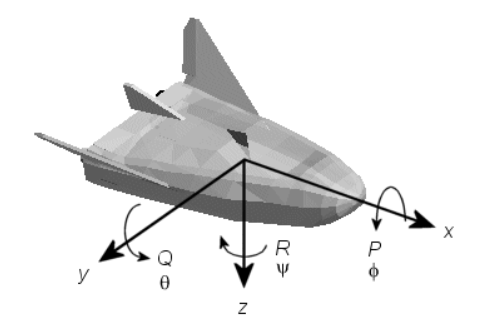
\includegraphics[width=\linewidth]{BodyFrame.png}
    \caption{Typical Body Frame Orientation}
    \label{fig:BodyFrameTypical}
\end{figure}

For our current model, the body frame of our 6-DoF has its origin in the nose of the vehicle. It has the first body basis vector, $\hat{X}$, pointing up along the longitudinal axis of the rocket following standard convention. The second basis vector, $\hat{Y}$, points right due East when on the launch pad, and the third, $\hat{Z}$, points due North on the launch pad. We use the cardinal directions of the launchpad as not only are there no conventional wings on the rocket, but it allows body frame to be defined parallel to the corresponding inertial frame basis vectors. Note that they won’t remain pointing in these directions as the rocket moves through space, and they may not even begin parallel to the inertial axis to begin with if the rocket launches from a tilt.

\begin{figure}[H]
\centering
\tikzset{every picture/.style={line width=0.75pt}} %set default line width to 0.75pt        

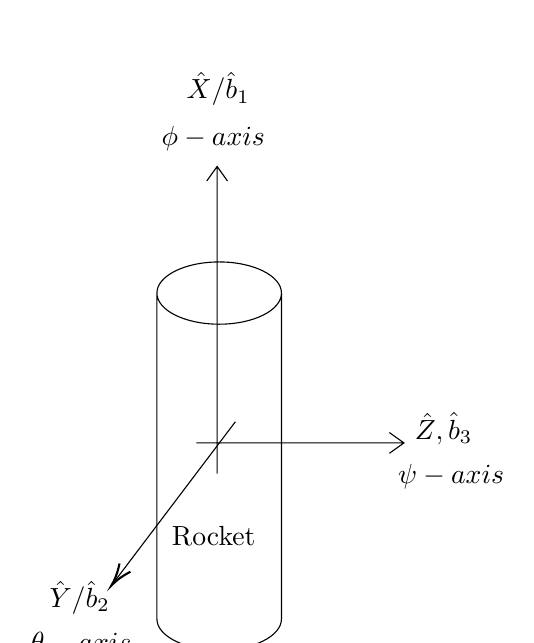
\begin{tikzpicture}[x=0.75pt,y=0.75pt,yscale=-1,xscale=1]
%uncomment if require: \path (0,408); %set diagram left start at 0, and has height of 408

%Shape: Can [id:dp7760621042562805] 
\draw   (351,111) -- (351,268) .. controls (351,276.28) and (337.57,283) .. (321,283) .. controls (304.43,283) and (291,276.28) .. (291,268) -- (291,111) .. controls (291,102.72) and (304.43,96) .. (321,96) .. controls (337.57,96) and (351,102.72) .. (351,111) .. controls (351,119.28) and (337.57,126) .. (321,126) .. controls (304.43,126) and (291,119.28) .. (291,111) ;
%Shape: Axis 2D [id:dp16563267347652144] 
\draw  (310,183.2) -- (410,183.2)(320,50) -- (320,198) (403,178.2) -- (410,183.2) -- (403,188.2) (315,57) -- (320,50) -- (325,57)  ;
%Straight Lines [id:da8489216589462083] 
\draw    (328.8,173) -- (270.21,250.41) ;
\draw [shift={(269,252)}, rotate = 307.12] [color={rgb, 255:red, 0; green, 0; blue, 0 }  ][line width=0.75]    (10.93,-3.29) .. controls (6.95,-1.4) and (3.31,-0.3) .. (0,0) .. controls (3.31,0.3) and (6.95,1.4) .. (10.93,3.29)   ;

% Text Node
\draw (304,3.4) node [anchor=north west][inner sep=0.75pt]    {$\hat{X} /\hat{b}_{1}$};
% Text Node
\draw (238,248.4) node [anchor=north west][inner sep=0.75pt]    {$\hat{Y} /\hat{b}_{2}$};
% Text Node
\draw (414,167.4) node [anchor=north west][inner sep=0.75pt]    {$\hat{Z} ,\hat{b}_{3}$};
% Text Node
\draw (297,222) node [anchor=north west][inner sep=0.75pt]   [align=left] {Rocket};
% Text Node
\draw (292,29.4) node [anchor=north west][inner sep=0.75pt]    {$\phi -axis$};
% Text Node
\draw (229,273.4) node [anchor=north west][inner sep=0.75pt]    {$\theta -axis$};
% Text Node
\draw (406,192.4) node [anchor=north west][inner sep=0.75pt]    {$\psi -axis$};

\end{tikzpicture}
    \caption{Body Frame Convention of our Rocket}
    \label{fig:BodyFrameRocket}
\end{figure}


%% Another Figure
\subsection{The Wind Frame}
The last and by far least important frame of reference is the \textit{wind frame.} This frame of reference, like the body frame, is always anchored at some point in the vehicle. Also like the body frame, it moves and rotates with the vehicle and allows for a new way of describing the state vector. Unlike the body frame, the most important definition is not along the longitudinal axis of the vehicle. As indicated by its name, the necessary orientation of a basis vector points in the direction of the free stream velocity. Relating this to the body frame, this translates to an offset from the body frame by the angle of attack and sideslip. This frame is often useful for aircraft, but we do not use it explicitly in our 6DoF. The wind frame itself is in fact skipped over during wind calculations, as the angle of attack and imparted forces/moments are calculated directly onto the body frame. So as this isn’t as useful as the other two reference frames, we won’t elaborate on this frame any further, and it won’t be shown as much in our example 6-DoF.

\newpage
\section{2-D Rotations}\label{sec:2D Rotations}
Before moving into 3-dimensional space, let’s start simple. Say you have an arrow drawn on a piece of paper, and you twist the paper about the origin of that arrow through an angle $\theta$. While you could measure the new vector’s components directly to describe your new arrow, we want a more generalized way to find a new vector for any rotation. 
\subsection{Real Rotations}
We will start the problem by defining our notation. We will utilize Cartesian coordinates with the positive $\hat{x}$ direction pointing to the right, $\hat{y}$ up, and $\hat{z}$ coming out of the page. Using this convention, a positive $\theta$ rotation is counterclockwise about the origin by use of the \textit{right hand rule (for rotations)}. We show an example of such a rotation in \ref{fig:2DRotation}:
%add glossary entry
\begin{figure}[H]
\centering

\tikzset{every picture/.style={line width=0.75pt}} %set default line width to 0.75pt        

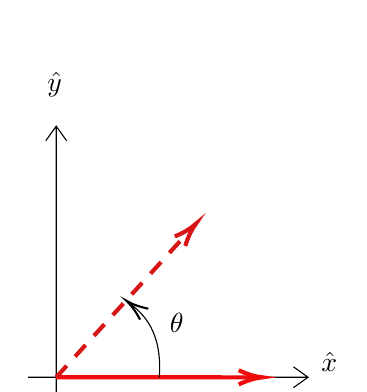
\begin{tikzpicture}[x=0.75pt,y=0.75pt,yscale=-1,xscale=1]
%uncomment if require: \path (0,300); %set diagram left start at 0, and has height of 300

%Shape: Axis 2D [id:dp2369017718792994] 
\draw  (274,169.56) -- (408.8,169.56)(287.48,48.6) -- (287.48,183) (401.8,164.56) -- (408.8,169.56) -- (401.8,174.56) (282.48,55.6) -- (287.48,48.6) -- (292.48,55.6)  ;
%Straight Lines [id:da6414021669220791] 
\draw [color={rgb, 255:red, 239; green, 11; blue, 11 }  ,draw opacity=1 ][line width=1.5]    (287.48,169.56) -- (383.8,169.6) ;
\draw [shift={(386.8,169.6)}, rotate = 180.02] [color={rgb, 255:red, 239; green, 11; blue, 11 }  ,draw opacity=1 ][line width=1.5]    (11.37,-3.42) .. controls (7.23,-1.45) and (3.44,-0.31) .. (0,0) .. controls (3.44,0.31) and (7.23,1.45) .. (11.37,3.42)   ;
%Straight Lines [id:da18731248462614536] 
\draw [color={rgb, 255:red, 215; green, 23; blue, 23 }  ,draw opacity=1 ][line width=1.5]  [dash pattern={on 5.63pt off 4.5pt}]  (287.48,169.56) -- (352.78,97.82) ;
\draw [shift={(354.8,95.6)}, rotate = 132.31] [color={rgb, 255:red, 215; green, 23; blue, 23 }  ,draw opacity=1 ][line width=1.5]    (11.37,-3.42) .. controls (7.23,-1.45) and (3.44,-0.31) .. (0,0) .. controls (3.44,0.31) and (7.23,1.45) .. (11.37,3.42)   ;
%Curve Lines [id:da22919468225468265] 
\draw    (337.14,169.58) .. controls (338.68,147.4) and (329.38,138.89) .. (322.7,133.77) ;
\draw [shift={(321.14,132.58)}, rotate = 37.01] [color={rgb, 255:red, 0; green, 0; blue, 0 }  ][line width=0.75]    (10.93,-3.29) .. controls (6.95,-1.4) and (3.31,-0.3) .. (0,0) .. controls (3.31,0.3) and (6.95,1.4) .. (10.93,3.29)   ;

% Text Node
\draw (341,137.4) node [anchor=north west][inner sep=0.75pt]    {$\theta $};
% Text Node
\draw (414,156.4) node [anchor=north west][inner sep=0.75pt]    {$\hat{x}$};
% Text Node
\draw (282,21.4) node [anchor=north west][inner sep=0.75pt]    {$\hat{y}$};


\end{tikzpicture}
    \caption{Example of 2-D Rotation}
    \label{fig:2DRotation}
\end{figure}
% do we want to use row vector when writing inline to make it cleaner?
In Figure \ref{fig:2DRotation}, our solid vector can be written as a column vector
$\begin{bmatrix}
    1\\0
\end{bmatrix}$, where the first element is the magnitude in the $\hat{x}$ direction and the second is the magnitude in the $\hat{y}$ direction.

With knowledge of linear algebra, we can see that the rotation of the vector is just some scaling and shearing of the original vector that preserves the vector length. These operations are \textit{linear}, so it is possible to find a matrix representation of this transformation.\footnote{We may also note that the property of preserving length means that our matrix must be \textit{unitary}. \textit{Unitary} matrices also preserve the inner product. Both of these are useful properties of these matrices. From these properties, it can also be shown that this matrix must be square.}

Mathematically, we want to find a square $2\times2$ matrix $R$ – called the rotation matrix – such that: $\vec{v}_2=R\vec{v}_1$
where $\vec{v}_1$ is our original vector, and $\vec{v}_2$ is our new, rotated vector. To derive our rotation matrix $R$, we will consider two similar vectors: our $\vec{v}_1$ mentioned above, as well as a new unit vector in the $\hat{y}$-direction 
$\begin{bmatrix}
    0\\1
\end{bmatrix}$.
For each of our unit vectors, we will use 90- and 180-degree rotations, since we know what solution we should acquire for each. Those being 
$\begin{bmatrix}
    0\\1
\end{bmatrix}$
and 
$\begin{bmatrix}
    -1\\0
\end{bmatrix}$
respectively for our first unit vector. 
Using the initial equation given above paired with our first 90-degree rotation, we get

$$\begin{bmatrix}
    0\\1
\end{bmatrix}=R
\begin{bmatrix}
    1\\0
\end{bmatrix}$$

Based off our knowledge of trigonometry, we already know that some combination of sines and cosines will construct our matrix $R$. With our choice of the $\hat{x}$-direction unit vector, only the first column of $R$, $\begin{bmatrix}
    r_{11}\\r_{21}
\end{bmatrix}$, will remain after matrix multiplication. This allows for the first column of $R$ to be solved as
$$\begin{bmatrix}
    0\\1
\end{bmatrix}=
\begin{bmatrix}
    r_{11}\\r_{21}
\end{bmatrix}
$$
And with a 90 degree rotation, $r_{21}$ can be determined to be $sin(\theta)$. Moving on to the second rotation, we use the equation 
$$\begin{bmatrix}
    -1\\0
\end{bmatrix}=R
\begin{bmatrix}
    1\\0
\end{bmatrix}$$
Repeating the above process, we get:
$$\begin{bmatrix}
    -1\\0
\end{bmatrix}=
\begin{bmatrix}
    r_{11}\\sin(\theta)
\end{bmatrix}$$
At a rotation of 180 degrees, $r_{11}$ must be $cos(\theta)$. We have now completed the first column of $R$: $\begin{bmatrix}
    cos(\theta)\\sin(\theta)
\end{bmatrix}$. If we plot the rotated unit vector as a function of $\theta$ from [0, 360) degrees, we can see that we do indeed get the unit circle.
For the $\hat{y}$ unit vector we follow an identical process and derive the second column of $R$. This derivation will be left as an exercise to the reader due to the redundancy and simplicity of the process; however, we end up with $\begin{bmatrix}
    -sin(\theta)\\cos(\theta)
\end{bmatrix}$ as our second column vector. Putting the two together, we have our completed rotation matrix \eqref{eq:2DMatrix}:
\begin{equation}\label{eq:2DMatrix}
    R=
    \begin{bmatrix}
        cos(\theta)&-sin(\theta)\\sin(\theta)&cos(\theta)
    \end{bmatrix}
\end{equation}
The understanding of this derivation is helpful to the understanding of the derivation of the rotation matrix in 3-dimensional space, so we will be sure to keep this process handy!

\subsection{Imaginary Rotations}
After deriving the matrix for rotations in regular 2-dimensional space, we can use this to describe the rotation of a vector in imaginary space. These results will serve as a basis for the motivation of quaternion rotations, which will be discussed later. 

To motive complex rotations, we will start with the famous Euler's Formula:
\begin{equation}
    e^{i\theta}=cos\theta+i\cdot sin\theta
\end{equation}
A succinct and intuitive explanation of Euler's Formula is given in two 3Blue1Brown videos, shown in sources \cite{3blue1brown_ei_2019} and \cite{3blue1brown_how_2021}. Because these videos so expertly describe this topic, we choose not to do so here. As an exercise to the reader, you can try proving this statement yourself by considering the Taylor Series expansion of $e^{ix}$ and comparing it with the Taylor Series of $sin(x)$ and $cos(x)$

So, since the magnitude of $e^{i\theta}$ is always 1, we can parameterize the length of our vector as its magnitude, $r$.

So, we now have a complex rotator which we can describe as:
\begin{gather}
    r=cos(\theta)+i\cdot sin(\theta)\\
    \text{or}\\
    r=e^{i\theta}
\end{gather}
This way, any rotation $\theta$ here is an identical to a rotation of the same  above, notation and all. We are simply replacing our x-axis with our real axis, and our y-axis with an imaginary axis. From this equality, we see that multiplication of a complex number corresponding to the appropriate real and imaginary components with the above complex rotator will result in an identical rotation to the same initial conditions in 2-dimensional space.

% we can add the other proof here as well if you want.

One thing to note here is that we can parameterize a rotation very cleanly and naturally with complex numbers. When we discuss quaternions in Section \ref{sec:quaternions}, these complex numbers will become increasingly important. 
\section{Euler Angles}
Now that we have reinforced our knowledge of reference frames and completed the simple 2-dimensional case of rotation, we are ready to move on to the significantly more complicated 3-dimensional case. There are two possible ways to describe a 3-dimensional rotation, with the first and more basic of the two being the method of \textit{Euler angles}.

Let’s say you’ve left the airport flying to Tahiti for vacation. While describing the translational motion of your aircraft is fairly simple, the orientation is much more difficult to determine. Euler angles give a systematic method of describing that orientation with respect to an inertial frame. While systematic, there are many ways to describe the same rotation. Taking the example of your aircraft banking and climbing away from the airport, the pilot is actively controlling the aircraft using the aircraft’s control surfaces. These combine to alter the yaw, pitch, and roll of the aircraft. When mathematically describing the orientation of the aircraft as a combination of these angles, the order both does and does not matter. While keeping the same order throughout calculations is incredibly important - which we will show in subsequent sections - the initial order you choose doesn’t matter nearly as much. So long as you don’t double up on rotations (e.g. two roll movements in a row) you can choose any order of rotation you want. This means there are a total of 12 possible rotation sequences (stemming from 3 frames to choose from x 2 frames not chosen immediately prior x 2 frames not chosen immediately prior = 12 sequences).

In industry and in academia, the 3-1-3 and 3-2-1 rotation orders are by far the most popular. Our example specifically uses the 3-2-1 rotation sequence due to its transparent connection with the traditional pitch, yaw, and roll maneuvers and subsequent uniqueness of a rotation-per-axis. We will use this option in our mathematical approaches throughout the rest of this section.

\subsection{3-D Rotations}

Like the 2-dimensional case before, we want to find a rotation matrix $R$ such that $\vec{v_2}=R\vec{v_1}$. Starting with our visualization, let’s say you now have a book laid flat on the table in front of you. We will now move through the two previously mentioned rotation sequences with that book: 3-2-1 and 3-1-3. Each of these individual rotations will be 90 degrees in the positive direction.
We will run through each sequence parallel to each other so any differences and similarities between the two can be easily visualized. You might want to grab a similar sized shape and follow along to aid in your understanding!

\begin{figure}[H]
\centering
\tikzset{every picture/.style={line width=0.75pt}} %set default line width to 0.75pt        
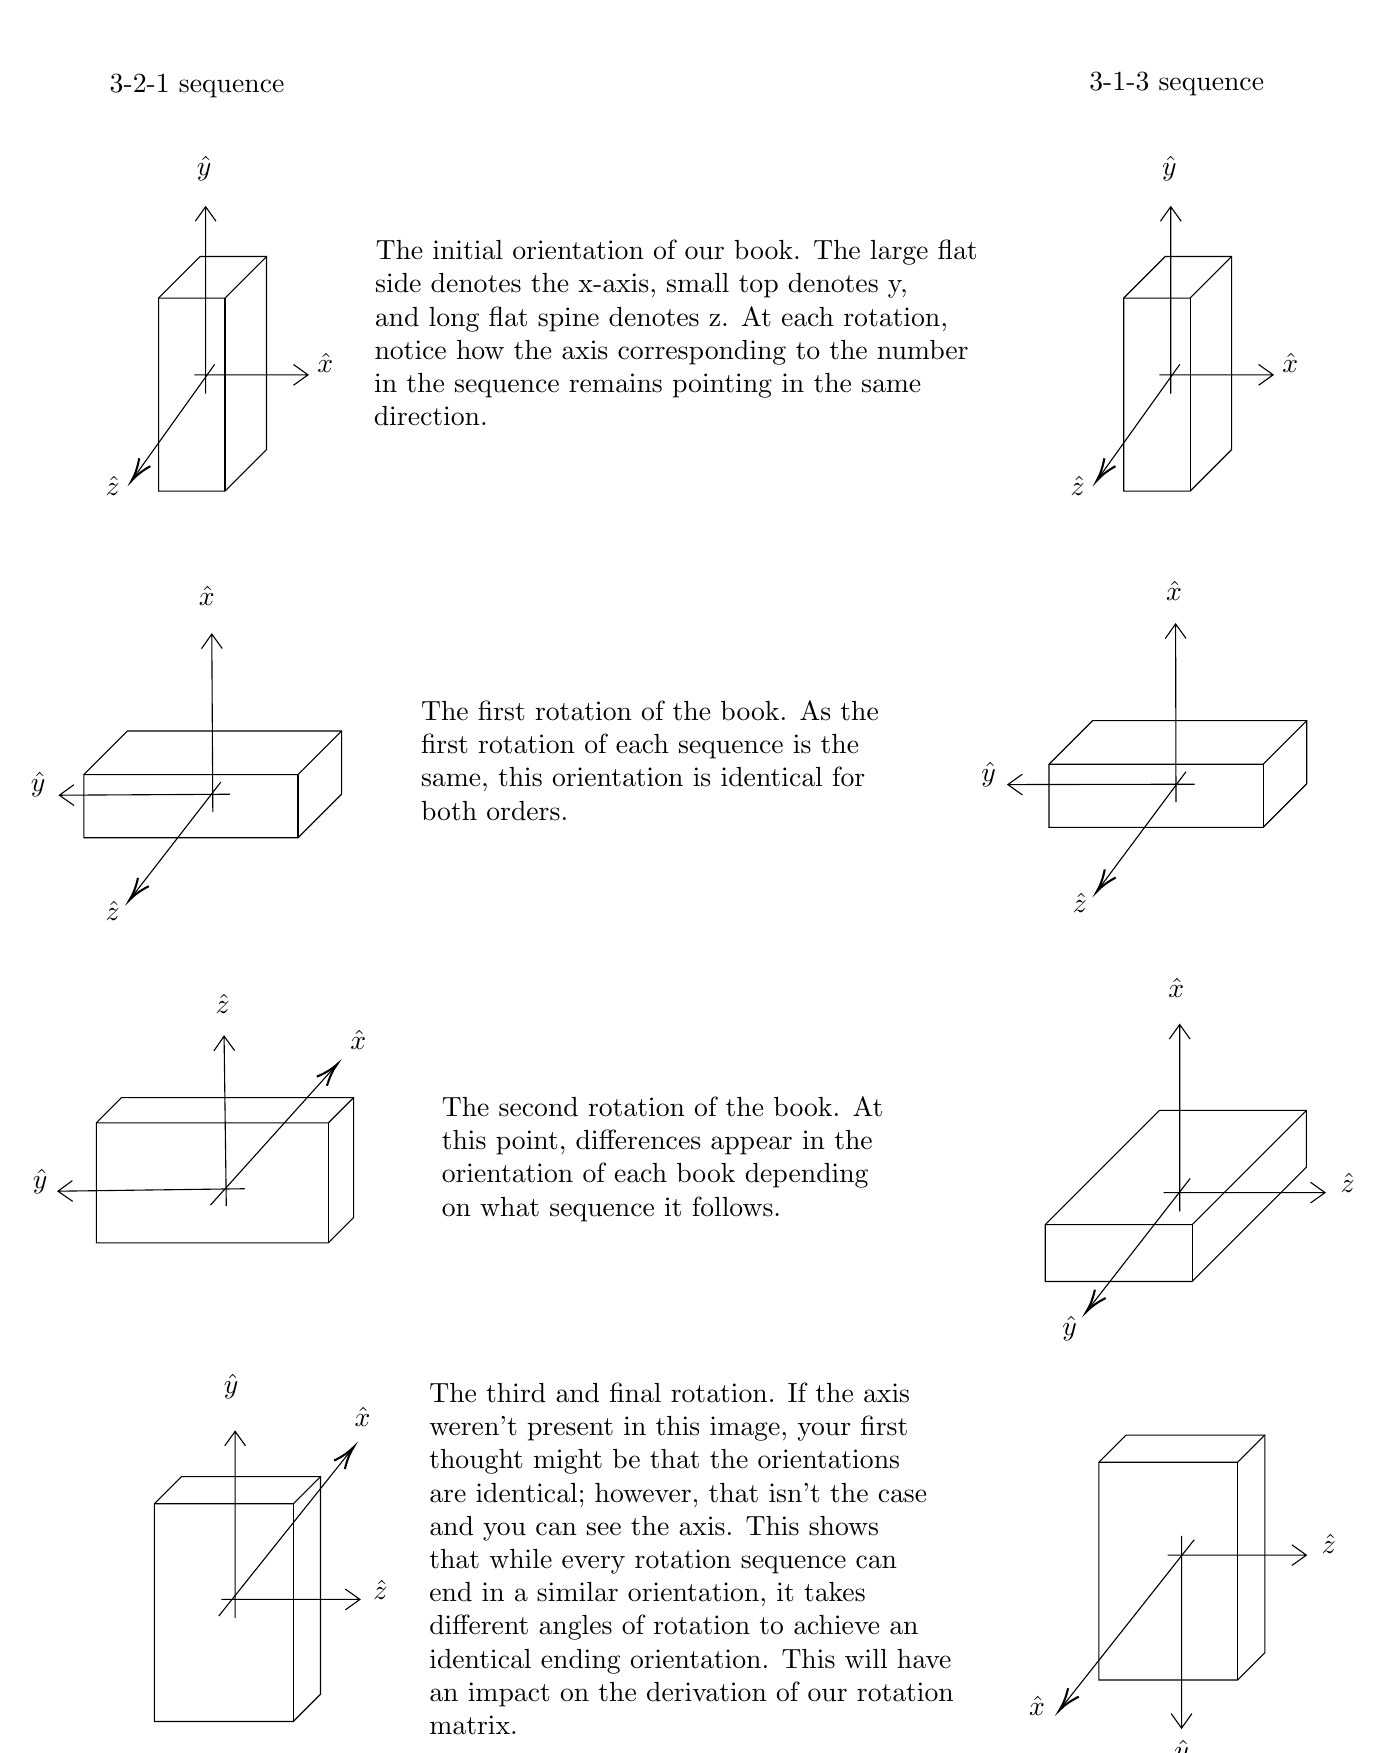
\begin{tikzpicture}[x=0.75pt,y=0.75pt,yscale=-1,xscale=1]
%uncomment if require: \path (0,898); %set diagram left start at 0, and has height of 898

%Shape: Cube [id:dp30473314642975957] 
\draw   (66.8,132) -- (86.8,112) -- (118.8,112) -- (118.8,205) -- (98.8,225) -- (66.8,225) -- cycle ; \draw   (118.8,112) -- (98.8,132) -- (66.8,132) ; \draw   (98.8,132) -- (98.8,225) ;
%Shape: Axis 2D [id:dp8167558306254183] 
\draw  (84,169) -- (138.8,169)(89.48,88) -- (89.48,178) (131.8,164) -- (138.8,169) -- (131.8,174) (84.48,95) -- (89.48,88) -- (94.48,95)  ;
%Straight Lines [id:da314709669225804] 
\draw    (93.8,164) -- (54.96,218.37) ;
\draw [shift={(53.8,220)}, rotate = 305.54] [color={rgb, 255:red, 0; green, 0; blue, 0 }  ][line width=0.75]    (10.93,-3.29) .. controls (6.95,-1.4) and (3.31,-0.3) .. (0,0) .. controls (3.31,0.3) and (6.95,1.4) .. (10.93,3.29)   ;
%Shape: Cube [id:dp04065664034078331] 
\draw   (531.8,132) -- (551.8,112) -- (583.8,112) -- (583.8,205) -- (563.8,225) -- (531.8,225) -- cycle ; \draw   (583.8,112) -- (563.8,132) -- (531.8,132) ; \draw   (563.8,132) -- (563.8,225) ;
%Shape: Axis 2D [id:dp3732351982959756] 
\draw  (549,169) -- (603.8,169)(554.48,88) -- (554.48,178) (596.8,164) -- (603.8,169) -- (596.8,174) (549.48,95) -- (554.48,88) -- (559.48,95)  ;
%Straight Lines [id:da7067184304168816] 
\draw    (558.8,164) -- (519.96,218.37) ;
\draw [shift={(518.8,220)}, rotate = 305.54] [color={rgb, 255:red, 0; green, 0; blue, 0 }  ][line width=0.75]    (10.93,-3.29) .. controls (6.95,-1.4) and (3.31,-0.3) .. (0,0) .. controls (3.31,0.3) and (6.95,1.4) .. (10.93,3.29)   ;
%Shape: Axis 2D [id:dp7824359400520153] 
\draw  (92.94,379.69) -- (92.44,293.89)(19.02,371.53) -- (101.1,371.06) (87.48,300.92) -- (92.44,293.89) -- (97.48,300.86) (26.05,376.49) -- (19.02,371.53) -- (25.99,366.49)  ;
%Straight Lines [id:da6575365467308292] 
\draw    (96.8,365.2) -- (54.02,420.42) ;
\draw [shift={(52.8,422)}, rotate = 307.76] [color={rgb, 255:red, 0; green, 0; blue, 0 }  ][line width=0.75]    (10.93,-3.29) .. controls (6.95,-1.4) and (3.31,-0.3) .. (0,0) .. controls (3.31,0.3) and (6.95,1.4) .. (10.93,3.29)   ;
%Shape: Axis 2D [id:dp26903333318867806] 
\draw  (97,759) -- (163.8,759)(103.68,678) -- (103.68,768) (156.8,754) -- (163.8,759) -- (156.8,764) (98.68,685) -- (103.68,678) -- (108.68,685)  ;
%Straight Lines [id:da6349794234163055] 
\draw    (95.8,767) -- (159.55,687.16) ;
\draw [shift={(160.8,685.6)}, rotate = 128.61] [color={rgb, 255:red, 0; green, 0; blue, 0 }  ][line width=0.75]    (10.93,-3.29) .. controls (6.95,-1.4) and (3.31,-0.3) .. (0,0) .. controls (3.31,0.3) and (6.95,1.4) .. (10.93,3.29)   ;
%Shape: Cube [id:dp3079853795797345] 
\draw   (30.8,361.6) -- (51.8,340.6) -- (155,340.6) -- (155,371) -- (134,392) -- (30.8,392) -- cycle ; \draw   (155,340.6) -- (134,361.6) -- (30.8,361.6) ; \draw   (134,361.6) -- (134,392) ;
%Shape: Axis 2D [id:dp9811912589376763] 
\draw  (556.99,374.82) -- (556.81,289.02)(475.97,366.41) -- (565.97,366.23) (551.82,296.04) -- (556.81,289.02) -- (561.82,296.01) (482.98,371.4) -- (475.97,366.41) -- (482.96,361.4)  ;
%Straight Lines [id:da8527731941171708] 
\draw    (561.8,360.2) -- (519.99,416.4) ;
\draw [shift={(518.8,418)}, rotate = 306.65] [color={rgb, 255:red, 0; green, 0; blue, 0 }  ][line width=0.75]    (10.93,-3.29) .. controls (6.95,-1.4) and (3.31,-0.3) .. (0,0) .. controls (3.31,0.3) and (6.95,1.4) .. (10.93,3.29)   ;
%Shape: Cube [id:dp41311458155167946] 
\draw   (495.8,356.6) -- (516.8,335.6) -- (620,335.6) -- (620,366) -- (599,387) -- (495.8,387) -- cycle ; \draw   (620,335.6) -- (599,356.6) -- (495.8,356.6) ; \draw   (599,356.6) -- (599,387) ;
%Shape: Axis 2D [id:dp09007049367762732] 
\draw  (551,563) -- (628.8,563)(558.78,482) -- (558.78,572) (621.8,558) -- (628.8,563) -- (621.8,568) (553.78,489) -- (558.78,482) -- (563.78,489)  ;
%Straight Lines [id:da7551423149111343] 
\draw    (563.8,556.2) -- (515.03,618.82) ;
\draw [shift={(513.8,620.4)}, rotate = 307.91] [color={rgb, 255:red, 0; green, 0; blue, 0 }  ][line width=0.75]    (10.93,-3.29) .. controls (6.95,-1.4) and (3.31,-0.3) .. (0,0) .. controls (3.31,0.3) and (6.95,1.4) .. (10.93,3.29)   ;
%Shape: Axis 2D [id:dp7930036978994484] 
\draw  (99.43,569.43) -- (98.36,487.63)(18.33,562.31) -- (108.32,561.13) (93.45,494.7) -- (98.36,487.63) -- (103.45,494.57) (25.4,567.21) -- (18.33,562.31) -- (25.27,557.22)  ;
%Straight Lines [id:da0514151325879022] 
\draw    (91.8,569) -- (151.46,502.69) ;
\draw [shift={(152.8,501.2)}, rotate = 131.98] [color={rgb, 255:red, 0; green, 0; blue, 0 }  ][line width=0.75]    (10.93,-3.29) .. controls (6.95,-1.4) and (3.31,-0.3) .. (0,0) .. controls (3.31,0.3) and (6.95,1.4) .. (10.93,3.29)   ;
%Shape: Cube [id:dp36832123870677336] 
\draw   (494,578.4) -- (549,523.4) -- (619.8,523.4) -- (619.8,550.8) -- (564.8,605.8) -- (494,605.8) -- cycle ; \draw   (619.8,523.4) -- (564.8,578.4) -- (494,578.4) ; \draw   (564.8,578.4) -- (564.8,605.8) ;
%Shape: Cube [id:dp9643780074556838] 
\draw   (36.8,529.4) -- (49,517.2) -- (160.8,517.2) -- (160.8,575) -- (148.6,587.2) -- (36.8,587.2) -- cycle ; \draw   (160.8,517.2) -- (148.6,529.4) -- (36.8,529.4) ; \draw   (148.6,529.4) -- (148.6,587.2) ;
%Shape: Cube [id:dp238953851849667] 
\draw   (64.8,712.9) -- (77.9,699.8) -- (144.8,699.8) -- (144.8,804.7) -- (131.7,817.8) -- (64.8,817.8) -- cycle ; \draw   (144.8,699.8) -- (131.7,712.9) -- (64.8,712.9) ; \draw   (131.7,712.9) -- (131.7,817.8) ;
%Shape: Axis 2D [id:dp7592681759502293] 
\draw  (553,737.66) -- (619.8,737.66)(559.68,821) -- (559.68,728.4) (612.8,742.66) -- (619.8,737.66) -- (612.8,732.66) (554.68,814) -- (559.68,821) -- (564.68,814)  ;
%Straight Lines [id:da36047739383645205] 
\draw    (565.8,730.2) -- (502.04,810.83) ;
\draw [shift={(500.8,812.4)}, rotate = 308.34] [color={rgb, 255:red, 0; green, 0; blue, 0 }  ][line width=0.75]    (10.93,-3.29) .. controls (6.95,-1.4) and (3.31,-0.3) .. (0,0) .. controls (3.31,0.3) and (6.95,1.4) .. (10.93,3.29)   ;
%Shape: Cube [id:dp22943768586952062] 
\draw   (519.8,692.9) -- (532.9,679.8) -- (599.8,679.8) -- (599.8,784.7) -- (586.7,797.8) -- (519.8,797.8) -- cycle ; \draw   (599.8,679.8) -- (586.7,692.9) -- (519.8,692.9) ; \draw   (586.7,692.9) -- (586.7,797.8) ;

% Text Node
\draw (142,157.4) node [anchor=north west][inner sep=0.75pt]    {$\hat{x}$};
% Text Node
\draw (84,62.4) node [anchor=north west][inner sep=0.75pt]    {$\hat{y}$};
% Text Node
\draw (40,216.4) node [anchor=north west][inner sep=0.75pt]    {$\hat{z}$};
% Text Node
\draw (170.17,103) node [anchor=north west][inner sep=0.75pt]  [xslant=0.01] [align=left] {The initial orientation of our book. The large flat \\side denotes the x-axis, small top denotes y, \\and long flat spine denotes z. At each rotation,\\notice how the axis corresponding to the number\\in the sequence remains pointing in the same\\direction.};
% Text Node
\draw (607,157.4) node [anchor=north west][inner sep=0.75pt]    {$\hat{x}$};
% Text Node
\draw (549,62.4) node [anchor=north west][inner sep=0.75pt]    {$\hat{y}$};
% Text Node
\draw (505,216.4) node [anchor=north west][inner sep=0.75pt]    {$\hat{z}$};
% Text Node
\draw (42,23) node [anchor=north west][inner sep=0.75pt]   [align=left] {3-2-1 sequence};
% Text Node
\draw (514,22) node [anchor=north west][inner sep=0.75pt]   [align=left] {3-1-3 sequence};
% Text Node
\draw (192,325) node [anchor=north west][inner sep=0.75pt]   [align=left] {The first rotation of the book. As the \\first rotation of each sequence is the \\same, this orientation is identical for \\both orders.};
% Text Node
\draw (85,269.4) node [anchor=north west][inner sep=0.75pt]    {$\hat{x}$};
% Text Node
\draw (4,359.4) node [anchor=north west][inner sep=0.75pt]    {$\hat{y}$};
% Text Node
\draw (40,421.4) node [anchor=north west][inner sep=0.75pt]    {$\hat{z}$};
% Text Node
\draw (160,665.4) node [anchor=north west][inner sep=0.75pt]    {$\hat{x}$};
% Text Node
\draw (97,649.4) node [anchor=north west][inner sep=0.75pt]    {$\hat{y}$};
% Text Node
\draw (169,748.4) node [anchor=north west][inner sep=0.75pt]    {$\hat{z}$};
% Text Node
\draw (551,267.4) node [anchor=north west][inner sep=0.75pt]    {$\hat{x}$};
% Text Node
\draw (462,354.4) node [anchor=north west][inner sep=0.75pt]    {$\hat{y}$};
% Text Node
\draw (506,417.4) node [anchor=north west][inner sep=0.75pt]    {$\hat{z}$};
% Text Node
\draw (202,515.8) node [anchor=north west][inner sep=0.75pt]   [align=left] {The second rotation of the book. At\\this point, differences appear in the\\orientation of each book depending\\on what sequence it follows.};
% Text Node
\draw (552,458.4) node [anchor=north west][inner sep=0.75pt]    {$\hat{x}$};
% Text Node
\draw (501,621.4) node [anchor=north west][inner sep=0.75pt]    {$\hat{y}$};
% Text Node
\draw (635,552.4) node [anchor=north west][inner sep=0.75pt]    {$\hat{z}$};
% Text Node
\draw (158,483.4) node [anchor=north west][inner sep=0.75pt]    {$\hat{x}$};
% Text Node
\draw (5,550.4) node [anchor=north west][inner sep=0.75pt]    {$\hat{y}$};
% Text Node
\draw (93,466.4) node [anchor=north west][inner sep=0.75pt]    {$\hat{z}$};
% Text Node
\draw (196,653.6) node [anchor=north west][inner sep=0.75pt]   [align=left] {The third and final rotation. If the axis \\weren't present in this image, your first\\thought might be that the orientations\\are identical; however, that isn't the case\\and you can see the axis. This shows\\that while every rotation sequence can\\end in a similar orientation, it takes \\different angles of rotation to achieve an\\identical ending orientation. This will have\\an impact on the derivation of our rotation\\matrix. };
% Text Node
\draw (485,804.4) node [anchor=north west][inner sep=0.75pt]    {$\hat{x}$};
% Text Node
\draw (555,825.4) node [anchor=north west][inner sep=0.75pt]    {$\hat{y}$};
% Text Node
\draw (626,726.4) node [anchor=north west][inner sep=0.75pt]    {$\hat{z}$};


\end{tikzpicture}
    \caption{Visualization of 3-Dimensional Rotation Sequences}
    \label{fig:3DParallelVisualization}
\end{figure}

Reinforcing the idea that different rotations are needed to achieve identical ending orientations for different rotation sequences, say you change the final 3-1-3 rotation to be -90 degrees. That ending orientation would now be perfectly identical to the 3-2-1 sequence! So despite what sequence you use, every possible ending orientation has the ability to be described by every rotation sequence, albeit with different individual angles of rotation. Now that we’ve seen the differences between the rotation sequences in the physical world, let’s try to describe them in the realm of mathematics. We will be following the 3-2-1 rotation sequence shown on the left of the image above. Like how we were able to visualize them above, we’re going to break each rotation down into smaller sets. In total we will go from the initial frame ($\hat{x}$,$\hat{y}$,$\hat{z}$), to the first intermediate frame (denoted by prime: $x'$), to the second intermediate frame (denoted by double prime: $x''$), to our final body frame ($\hat{X}$,$\hat{Y}$,$\hat{Z}$).
$$(\hat{x},\hat{y},\hat{z})\rightarrow(\hat{x}',\hat{y}',\hat{z}')\rightarrow(\hat{x}'',\hat{y}'',\hat{z}'')\rightarrow(\hat{X},\hat{Y},\hat{Z})$$

Having broken the big picture down into smaller, simpler ones, we can see that this daunting manipulation of the vehicle’s orientation in 3-dimensional space is merely a set of three simple 2-dimensional rotations in a set sequence (a fact heavily implied by the spatial manipulation of the textbook earlier!). The Euler Angles correspond to a 2-dimensional rotation about a paired axis. Our angle $\psi$ pairs with the z-axis and typically corresponds to the yaw of an aircraft, $\theta$ pairs with the y-axis and the pitch, while $\phi$ pairs with the x-axis and the roll. Images \ref{fig:BodyFrameTypical} and \ref{fig:BodyFrameRocket} reflect this, visualizing the standard and specific conventions for such a notation.

Utilizing this information and recalling our rotation matrix from 2-dimensional space \eqref{eq:2DMatrix} we can expand to 3-dimensional space. Our angle $\psi$, with it’s connection to the z-axis needs that axis to remain “stationary”. Therefore, the third component of the vector we are rotating about will always be multiplied by 1. Before throwing this in a matrix, let’s double check the rotation matrix for a vector also applies for the rotation of a frame.

Visualizing the rotation of the prime frame with respect to the initial frame by an angle $\psi$ about the z-axis, we get:

\begin{figure}[H]
\centering

\tikzset{every picture/.style={line width=0.75pt}} %set default line width to 0.75pt        

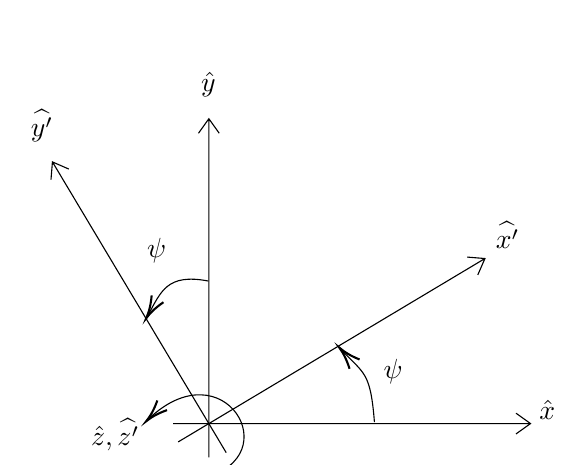
\begin{tikzpicture}[x=0.75pt,y=0.75pt,yscale=-1,xscale=1]
%uncomment if require: \path (0,300); %set diagram left start at 0, and has height of 300

%Shape: Axis 2D [id:dp8814120358250415] 
\draw  (294.8,194.88) -- (467,194.88)(312.02,48) -- (312.02,211.2) (460,189.88) -- (467,194.88) -- (460,199.88) (307.02,55) -- (312.02,48) -- (317.02,55)  ;
%Shape: Axis 2D [id:dp1264953723655049] 
\draw  (297.24,203.72) -- (445.04,115.36)(236.66,68.81) -- (320.39,208.89) (436.47,114.66) -- (445.04,115.36) -- (441.6,123.24) (235.96,77.38) -- (236.66,68.81) -- (244.54,72.25)  ;
%Curve Lines [id:da4379409407097825] 
\draw    (391.8,194.2) .. controls (389.87,170.07) and (387.01,171.09) .. (376.03,159.51) ;
\draw [shift={(374.8,158.2)}, rotate = 47.29] [color={rgb, 255:red, 0; green, 0; blue, 0 }  ][line width=0.75]    (10.93,-3.29) .. controls (6.95,-1.4) and (3.31,-0.3) .. (0,0) .. controls (3.31,0.3) and (6.95,1.4) .. (10.93,3.29)   ;
%Curve Lines [id:da47080870387004614] 
\draw    (311.8,126.2) .. controls (291.74,122.38) and (289.02,131.33) .. (282.72,142.59) ;
\draw [shift={(281.8,144.2)}, rotate = 300.26] [color={rgb, 255:red, 0; green, 0; blue, 0 }  ][line width=0.75]    (10.93,-3.29) .. controls (6.95,-1.4) and (3.31,-0.3) .. (0,0) .. controls (3.31,0.3) and (6.95,1.4) .. (10.93,3.29)   ;
%Curve Lines [id:da40076953586454556] 
\draw    (309.8,220.8) .. controls (350.39,210.9) and (319.43,157.88) .. (282.91,192.72) ;
\draw [shift={(281.8,193.8)}, rotate = 315] [color={rgb, 255:red, 0; green, 0; blue, 0 }  ][line width=0.75]    (10.93,-3.29) .. controls (6.95,-1.4) and (3.31,-0.3) .. (0,0) .. controls (3.31,0.3) and (6.95,1.4) .. (10.93,3.29)   ;

% Text Node
\draw (470,182.4) node [anchor=north west][inner sep=0.75pt]    {$\hat{x}$};
% Text Node
\draw (307,24.4) node [anchor=north west][inner sep=0.75pt]    {$\hat{y}$};
% Text Node
\draw (449,96.4) node [anchor=north west][inner sep=0.75pt]    {$\widehat{x'}$};
% Text Node
\draw (225,42.4) node [anchor=north west][inner sep=0.75pt]    {$\widehat{y'}$};
% Text Node
\draw (281,104.4) node [anchor=north west][inner sep=0.75pt]    {$\psi $};
% Text Node
\draw (395,162.4) node [anchor=north west][inner sep=0.75pt]    {$\psi $};
% Text Node
\draw (254,191.4) node [anchor=north west][inner sep=0.75pt]    {$\hat{z} ,\widehat{z'}$};

\end{tikzpicture}
   
    \caption{First Frame Rotation in 3-2-1 Sequence}
    \label{fig:3DZRotation}
\end{figure}

Computing the trigonometry to translate from the initial to prime frame, we get the following set of equations:
$$\hat{x}'=cos(\psi)\hat{x}+sin(\psi)\hat{y}$$
$$\hat{y}'=-sin(\psi)\hat{x}+cos(\psi)\hat{y}$$
$$\hat{z}'=\hat{z}$$
Concatenating these into a single matrix, we get the following rotation matrix about the z-axis in 3-dimensional space for a 3-2-1 rotation:
\begin{equation}\label{eq:3DZMatrix}
R(\psi)=\begin{bmatrix}
    cos(\psi)&sin(\psi)&0\\-sin(\psi)&cos(\psi)&0\\0&0&1
\end{bmatrix}
\end{equation}
We can see this matrix is in fact different from our 2-dimensional rotation matrix! The reason for this stems from the fact that while in 2-dimensions, we were rotating a vector, we are now rotating an entire frame at once in 3-dimensions. This difference has a subtle impact on the trigonometry of the problem, leading to the negative sine term switching across the diagonal. Performing the same process for our y-axis ($\theta$) we get the image and equations shown below:

\begin{figure}[H]
    
\centering

\tikzset{every picture/.style={line width=0.75pt}} %set default line width to 0.75pt        

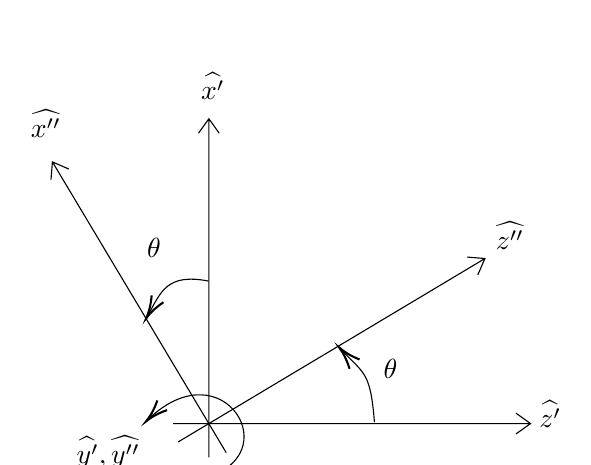
\begin{tikzpicture}[x=0.75pt,y=0.75pt,yscale=-1,xscale=1]
%uncomment if require: \path (0,300); %set diagram left start at 0, and has height of 300

%Shape: Axis 2D [id:dp10624606154766014] 
\draw  (289.8,225.88) -- (462,225.88)(307.02,79) -- (307.02,242.2) (455,220.88) -- (462,225.88) -- (455,230.88) (302.02,86) -- (307.02,79) -- (312.02,86)  ;
%Shape: Axis 2D [id:dp07151631286404303] 
\draw  (292.24,234.72) -- (440.04,146.36)(231.66,99.81) -- (315.39,239.89) (431.47,145.66) -- (440.04,146.36) -- (436.6,154.24) (230.96,108.38) -- (231.66,99.81) -- (239.54,103.25)  ;
%Curve Lines [id:da006532196783956223] 
\draw    (386.8,225.2) .. controls (384.87,201.07) and (382.01,202.09) .. (371.03,190.51) ;
\draw [shift={(369.8,189.2)}, rotate = 47.29] [color={rgb, 255:red, 0; green, 0; blue, 0 }  ][line width=0.75]    (10.93,-3.29) .. controls (6.95,-1.4) and (3.31,-0.3) .. (0,0) .. controls (3.31,0.3) and (6.95,1.4) .. (10.93,3.29)   ;
%Curve Lines [id:da19094795610816706] 
\draw    (306.8,157.2) .. controls (286.74,153.38) and (284.02,162.33) .. (277.72,173.59) ;
\draw [shift={(276.8,175.2)}, rotate = 300.26] [color={rgb, 255:red, 0; green, 0; blue, 0 }  ][line width=0.75]    (10.93,-3.29) .. controls (6.95,-1.4) and (3.31,-0.3) .. (0,0) .. controls (3.31,0.3) and (6.95,1.4) .. (10.93,3.29)   ;
%Curve Lines [id:da8842649250634054] 
\draw    (304.8,251.8) .. controls (345.39,241.9) and (314.43,188.88) .. (277.91,223.72) ;
\draw [shift={(276.8,224.8)}, rotate = 315] [color={rgb, 255:red, 0; green, 0; blue, 0 }  ][line width=0.75]    (10.93,-3.29) .. controls (6.95,-1.4) and (3.31,-0.3) .. (0,0) .. controls (3.31,0.3) and (6.95,1.4) .. (10.93,3.29)   ;

% Text Node
\draw (465,213.4) node [anchor=north west][inner sep=0.75pt]    {$\widehat{z'}$};
% Text Node
\draw (302,55.4) node [anchor=north west][inner sep=0.75pt]    {$\widehat{x'}$};
% Text Node
\draw (444,127.4) node [anchor=north west][inner sep=0.75pt]    {$\widehat{z''}$};
% Text Node
\draw (220,73.4) node [anchor=north west][inner sep=0.75pt]    {$\widehat{x''}$};
% Text Node
\draw (276,135.4) node [anchor=north west][inner sep=0.75pt]    {$\theta $};
% Text Node
\draw (390,193.4) node [anchor=north west][inner sep=0.75pt]    {$\theta $};
% Text Node
\draw (242,230.4) node [anchor=north west][inner sep=0.75pt]    {$\widehat{y'} ,\widehat{y''}$};


\end{tikzpicture}

    \caption{Second Frame Rotation in 3-2-1 Sequence}
    \label{fig:3DYRotation}

\end{figure}
$$\hat{x}''=cos(\theta)\hat{x}'-sin(\theta)\hat{z}'$$
$$\hat{y}''=\hat{y}'$$
$$\hat{z}''=sin(\theta)\hat{x}'+cos(\theta)\hat{z}'$$
And finally the matrix:
$$R(\theta)=\begin{bmatrix}
    cos(\theta)&0&-sin(\theta)\\0&1&0\\sin(\theta)&0&cos(\theta)
\end{bmatrix}$$
Finally for our x-axis ($\phi$), we get the image and equation below:

\begin{figure}[H]
    \centering

\tikzset{every picture/.style={line width=0.75pt}} %set default line width to 0.75pt        

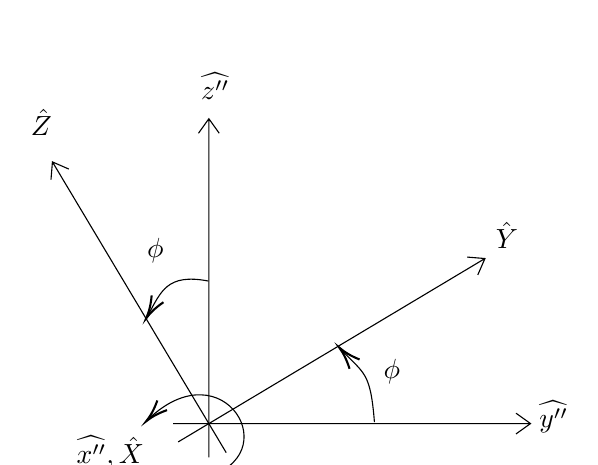
\begin{tikzpicture}[x=0.75pt,y=0.75pt,yscale=-1,xscale=1]
%uncomment if require: \path (0,300); %set diagram left start at 0, and has height of 300

%Shape: Axis 2D [id:dp37741929808299357] 
\draw  (265.8,214.88) -- (438,214.88)(283.02,68) -- (283.02,231.2) (431,209.88) -- (438,214.88) -- (431,219.88) (278.02,75) -- (283.02,68) -- (288.02,75)  ;
%Shape: Axis 2D [id:dp4057280236537508] 
\draw  (268.24,223.72) -- (416.04,135.36)(207.66,88.81) -- (291.39,228.89) (407.47,134.66) -- (416.04,135.36) -- (412.6,143.24) (206.96,97.38) -- (207.66,88.81) -- (215.54,92.25)  ;
%Curve Lines [id:da7885616787760448] 
\draw    (362.8,214.2) .. controls (360.87,190.07) and (358.01,191.09) .. (347.03,179.51) ;
\draw [shift={(345.8,178.2)}, rotate = 47.29] [color={rgb, 255:red, 0; green, 0; blue, 0 }  ][line width=0.75]    (10.93,-3.29) .. controls (6.95,-1.4) and (3.31,-0.3) .. (0,0) .. controls (3.31,0.3) and (6.95,1.4) .. (10.93,3.29)   ;
%Curve Lines [id:da4316718282657035] 
\draw    (282.8,146.2) .. controls (262.74,142.38) and (260.02,151.33) .. (253.72,162.59) ;
\draw [shift={(252.8,164.2)}, rotate = 300.26] [color={rgb, 255:red, 0; green, 0; blue, 0 }  ][line width=0.75]    (10.93,-3.29) .. controls (6.95,-1.4) and (3.31,-0.3) .. (0,0) .. controls (3.31,0.3) and (6.95,1.4) .. (10.93,3.29)   ;
%Curve Lines [id:da8810661168844911] 
\draw    (280.8,240.8) .. controls (321.39,230.9) and (290.43,177.88) .. (253.91,212.72) ;
\draw [shift={(252.8,213.8)}, rotate = 315] [color={rgb, 255:red, 0; green, 0; blue, 0 }  ][line width=0.75]    (10.93,-3.29) .. controls (6.95,-1.4) and (3.31,-0.3) .. (0,0) .. controls (3.31,0.3) and (6.95,1.4) .. (10.93,3.29)   ;

% Text Node
\draw (441,202.4) node [anchor=north west][inner sep=0.75pt]    {$\widehat{y''}$};
% Text Node
\draw (278,44.4) node [anchor=north west][inner sep=0.75pt]    {$\widehat{z''}$};
% Text Node
\draw (420,116.4) node [anchor=north west][inner sep=0.75pt]    {$\hat{Y}$};
% Text Node
\draw (196,62.4) node [anchor=north west][inner sep=0.75pt]    {$\hat{Z}$};
% Text Node
\draw (252,124.4) node [anchor=north west][inner sep=0.75pt]    {$\phi $};
% Text Node
\draw (366,182.4) node [anchor=north west][inner sep=0.75pt]    {$\phi $};
% Text Node
\draw (218,219.4) node [anchor=north west][inner sep=0.75pt]    {$\widehat{x''} ,\hat{X}$};


\end{tikzpicture}
    \caption{Final Frame Rotation in 3-2-1 Sequence}
    \label{fig:3DXRotation}
\end{figure}
$$\hat{X}=\hat{x}''$$
$$\hat{Y}=cos(\phi)\hat{y}''+sin(\phi)\hat{z}''$$
$$\hat{Z}=-sin(\phi)\hat{y}''+cos(\phi)\hat{z}''$$
And finally our last matrix:
$$R(\phi)=\begin{bmatrix}
    1&0&0\\0&cos(\phi)&sin(\phi)\\0&-sin(\phi)&cos(\phi)
\end{bmatrix}$$
Note it is VERY important to derive the individual rotation matrices with simple trigonometry for each axis if you choose a different rotation sequence, as the terms of each element in the matrix elements may change depending on what you do!

\subsection{The Direction Cosine Matrix}
Having matrices for each individual rotation is a great start; however, we want to get to the form:
$$\vec{R}=A_{3,2,1}\vec{r}$$
The 3x3 matrix $A_{3,2,1}$ is the \textit{Direction Cosine Matrix} or \textit{DCM}. This is the final, 3-dimensional rotation matrix you multiply with your inertial vector to express any vector in your body frame. Intuitively, we can presume the DCM will be some matrix multiplication of the three individual rotations. But in what order do we multiply our individual axis rotation matrices together? Remember, order matters in matrix multiplication as it is NOT commutative. So, determining the proper order is essential to the accuracy of the equation.

To work through this, we’re going to fall back on the tried-and-true method of visualization. Looking back at the image of our book, we’re going to replace the book with only the axis. The following set of images moves through these rotations; however, on a 2-dimensional piece of paper it’s a bit difficult to depict a 3-dimensional rotation.

\begin{figure}[H]
\centering



\tikzset{every picture/.style={line width=0.75pt}} %set default line width to 0.75pt        

\begin{tikzpicture}[x=0.75pt,y=0.75pt,yscale=-1,xscale=1]
%uncomment if require: \path (0,923); %set diagram left start at 0, and has height of 923

%Shape: Axis 2D [id:dp169089929067181] 
\draw  (119,117) -- (219,117)(129,27) -- (129,127) (212,112) -- (219,117) -- (212,122) (124,34) -- (129,27) -- (134,34)  ;
%Straight Lines [id:da807678379259174] 
\draw    (136.8,110.4) -- (78.26,165.04) ;
\draw [shift={(76.8,166.4)}, rotate = 316.97] [color={rgb, 255:red, 0; green, 0; blue, 0 }  ][line width=0.75]    (10.93,-3.29) .. controls (6.95,-1.4) and (3.31,-0.3) .. (0,0) .. controls (3.31,0.3) and (6.95,1.4) .. (10.93,3.29)   ;
%Shape: Axis 2D [id:dp7622456541943443] 
\draw  (123,323) -- (223,323)(133,233) -- (133,333) (216,318) -- (223,323) -- (216,328) (128,240) -- (133,233) -- (138,240)  ;
%Straight Lines [id:da7627359224242283] 
\draw    (140.8,316.4) -- (82.26,371.04) ;
\draw [shift={(80.8,372.4)}, rotate = 316.97] [color={rgb, 255:red, 0; green, 0; blue, 0 }  ][line width=0.75]    (10.93,-3.29) .. controls (6.95,-1.4) and (3.31,-0.3) .. (0,0) .. controls (3.31,0.3) and (6.95,1.4) .. (10.93,3.29)   ;
%Straight Lines [id:da9944755330031119] 
\draw    (133,323) -- (219.8,323.2) ;
\draw [shift={(221.8,323.2)}, rotate = 180.13] [color={rgb, 255:red, 0; green, 0; blue, 0 }  ][line width=0.75]    (10.93,-3.29) .. controls (6.95,-1.4) and (3.31,-0.3) .. (0,0) .. controls (3.31,0.3) and (6.95,1.4) .. (10.93,3.29)   ;
%Straight Lines [id:da8159551049186013] 
\draw    (140,333) -- (85.91,251.86) ;
\draw [shift={(84.8,250.2)}, rotate = 56.31] [color={rgb, 255:red, 0; green, 0; blue, 0 }  ][line width=0.75]    (10.93,-3.29) .. controls (6.95,-1.4) and (3.31,-0.3) .. (0,0) .. controls (3.31,0.3) and (6.95,1.4) .. (10.93,3.29)   ;
%Straight Lines [id:da2841054255340081] 
\draw    (135.8,314.2) -- (101.53,401.34) ;
\draw [shift={(100.8,403.2)}, rotate = 291.47] [color={rgb, 255:red, 0; green, 0; blue, 0 }  ][line width=0.75]    (10.93,-3.29) .. controls (6.95,-1.4) and (3.31,-0.3) .. (0,0) .. controls (3.31,0.3) and (6.95,1.4) .. (10.93,3.29)   ;
%Curve Lines [id:da4204693895037821] 
\draw    (131,271) .. controls (119.29,265.43) and (114.21,268.9) .. (107.63,281.57) ;
\draw [shift={(106.8,283.2)}, rotate = 296.57] [color={rgb, 255:red, 0; green, 0; blue, 0 }  ][line width=0.75]    (10.93,-3.29) .. controls (6.95,-1.4) and (3.31,-0.3) .. (0,0) .. controls (3.31,0.3) and (6.95,1.4) .. (10.93,3.29)   ;
%Curve Lines [id:da10253203244713682] 
\draw    (101.8,353.2) .. controls (98.9,365.74) and (98.8,370.84) .. (114.98,364.89) ;
\draw [shift={(116.8,364.2)}, rotate = 158.75] [color={rgb, 255:red, 0; green, 0; blue, 0 }  ][line width=0.75]    (10.93,-3.29) .. controls (6.95,-1.4) and (3.31,-0.3) .. (0,0) .. controls (3.31,0.3) and (6.95,1.4) .. (10.93,3.29)   ;
%Straight Lines [id:da8112981285659084] 
\draw    (371,323) -- (457.8,323.2) ;
\draw [shift={(459.8,323.2)}, rotate = 180.13] [color={rgb, 255:red, 0; green, 0; blue, 0 }  ][line width=0.75]    (10.93,-3.29) .. controls (6.95,-1.4) and (3.31,-0.3) .. (0,0) .. controls (3.31,0.3) and (6.95,1.4) .. (10.93,3.29)   ;
%Straight Lines [id:da22117378034771829] 
\draw    (385,331) -- (330.91,249.86) ;
\draw [shift={(329.8,248.2)}, rotate = 56.31] [color={rgb, 255:red, 0; green, 0; blue, 0 }  ][line width=0.75]    (10.93,-3.29) .. controls (6.95,-1.4) and (3.31,-0.3) .. (0,0) .. controls (3.31,0.3) and (6.95,1.4) .. (10.93,3.29)   ;
%Straight Lines [id:da6076277803798291] 
\draw    (381.8,315.2) -- (347.53,402.34) ;
\draw [shift={(346.8,404.2)}, rotate = 291.47] [color={rgb, 255:red, 0; green, 0; blue, 0 }  ][line width=0.75]    (10.93,-3.29) .. controls (6.95,-1.4) and (3.31,-0.3) .. (0,0) .. controls (3.31,0.3) and (6.95,1.4) .. (10.93,3.29)   ;
%Straight Lines [id:da22428135782433367] 
\draw    (133,556) -- (219.8,556.2) ;
\draw [shift={(221.8,556.2)}, rotate = 180.13] [color={rgb, 255:red, 0; green, 0; blue, 0 }  ][line width=0.75]    (10.93,-3.29) .. controls (6.95,-1.4) and (3.31,-0.3) .. (0,0) .. controls (3.31,0.3) and (6.95,1.4) .. (10.93,3.29)   ;
%Straight Lines [id:da6183300172376611] 
\draw    (147,564) -- (92.91,482.86) ;
\draw [shift={(91.8,481.2)}, rotate = 56.31] [color={rgb, 255:red, 0; green, 0; blue, 0 }  ][line width=0.75]    (10.93,-3.29) .. controls (6.95,-1.4) and (3.31,-0.3) .. (0,0) .. controls (3.31,0.3) and (6.95,1.4) .. (10.93,3.29)   ;
%Straight Lines [id:da7023296453623051] 
\draw    (143.8,548.2) -- (109.53,635.34) ;
\draw [shift={(108.8,637.2)}, rotate = 291.47] [color={rgb, 255:red, 0; green, 0; blue, 0 }  ][line width=0.75]    (10.93,-3.29) .. controls (6.95,-1.4) and (3.31,-0.3) .. (0,0) .. controls (3.31,0.3) and (6.95,1.4) .. (10.93,3.29)   ;
%Straight Lines [id:da8491036796335945] 
\draw    (152,561.8) -- (64.56,514.35) ;
\draw [shift={(62.8,513.4)}, rotate = 28.48] [color={rgb, 255:red, 0; green, 0; blue, 0 }  ][line width=0.75]    (10.93,-3.29) .. controls (6.95,-1.4) and (3.31,-0.3) .. (0,0) .. controls (3.31,0.3) and (6.95,1.4) .. (10.93,3.29)   ;
%Straight Lines [id:da9327416644156861] 
\draw    (131,563.8) -- (202.17,513.55) ;
\draw [shift={(203.8,512.4)}, rotate = 144.78] [color={rgb, 255:red, 0; green, 0; blue, 0 }  ][line width=0.75]    (10.93,-3.29) .. controls (6.95,-1.4) and (3.31,-0.3) .. (0,0) .. controls (3.31,0.3) and (6.95,1.4) .. (10.93,3.29)   ;
%Curve Lines [id:da18651531365927365] 
\draw    (186,556.8) .. controls (205.76,538.37) and (194.11,532.94) .. (182.61,529.01) ;
\draw [shift={(180.8,528.4)}, rotate = 18.43] [color={rgb, 255:red, 0; green, 0; blue, 0 }  ][line width=0.75]    (10.93,-3.29) .. controls (6.95,-1.4) and (3.31,-0.3) .. (0,0) .. controls (3.31,0.3) and (6.95,1.4) .. (10.93,3.29)   ;
%Curve Lines [id:da031042459135772082] 
\draw    (114,512.8) .. controls (99.48,516.24) and (97.92,517.3) .. (95.19,529.59) ;
\draw [shift={(94.8,531.4)}, rotate = 282.09] [color={rgb, 255:red, 0; green, 0; blue, 0 }  ][line width=0.75]    (10.93,-3.29) .. controls (6.95,-1.4) and (3.31,-0.3) .. (0,0) .. controls (3.31,0.3) and (6.95,1.4) .. (10.93,3.29)   ;
%Straight Lines [id:da8477850498962038] 
\draw    (389.8,552.2) -- (355.53,639.34) ;
\draw [shift={(354.8,641.2)}, rotate = 291.47] [color={rgb, 255:red, 0; green, 0; blue, 0 }  ][line width=0.75]    (10.93,-3.29) .. controls (6.95,-1.4) and (3.31,-0.3) .. (0,0) .. controls (3.31,0.3) and (6.95,1.4) .. (10.93,3.29)   ;
%Straight Lines [id:da8683274216475789] 
\draw    (395,562.8) -- (307.56,515.35) ;
\draw [shift={(305.8,514.4)}, rotate = 28.48] [color={rgb, 255:red, 0; green, 0; blue, 0 }  ][line width=0.75]    (10.93,-3.29) .. controls (6.95,-1.4) and (3.31,-0.3) .. (0,0) .. controls (3.31,0.3) and (6.95,1.4) .. (10.93,3.29)   ;
%Straight Lines [id:da6438781119062607] 
\draw    (380,564.8) -- (451.17,514.55) ;
\draw [shift={(452.8,513.4)}, rotate = 144.78] [color={rgb, 255:red, 0; green, 0; blue, 0 }  ][line width=0.75]    (10.93,-3.29) .. controls (6.95,-1.4) and (3.31,-0.3) .. (0,0) .. controls (3.31,0.3) and (6.95,1.4) .. (10.93,3.29)   ;
%Straight Lines [id:da784757290818016] 
\draw    (135.8,773.2) -- (101.53,860.34) ;
\draw [shift={(100.8,862.2)}, rotate = 291.47] [color={rgb, 255:red, 0; green, 0; blue, 0 }  ][line width=0.75]    (10.93,-3.29) .. controls (6.95,-1.4) and (3.31,-0.3) .. (0,0) .. controls (3.31,0.3) and (6.95,1.4) .. (10.93,3.29)   ;
%Straight Lines [id:da5207150108611938] 
\draw    (141,783.8) -- (53.56,736.35) ;
\draw [shift={(51.8,735.4)}, rotate = 28.48] [color={rgb, 255:red, 0; green, 0; blue, 0 }  ][line width=0.75]    (10.93,-3.29) .. controls (6.95,-1.4) and (3.31,-0.3) .. (0,0) .. controls (3.31,0.3) and (6.95,1.4) .. (10.93,3.29)   ;
%Straight Lines [id:da3827560154389007] 
\draw    (126,785.8) -- (197.17,735.55) ;
\draw [shift={(198.8,734.4)}, rotate = 144.78] [color={rgb, 255:red, 0; green, 0; blue, 0 }  ][line width=0.75]    (10.93,-3.29) .. controls (6.95,-1.4) and (3.31,-0.3) .. (0,0) .. controls (3.31,0.3) and (6.95,1.4) .. (10.93,3.29)   ;
%Straight Lines [id:da7174569054516935] 
\draw    (126,792) -- (177.7,713.27) ;
\draw [shift={(178.8,711.6)}, rotate = 123.29] [color={rgb, 255:red, 0; green, 0; blue, 0 }  ][line width=0.75]    (10.93,-3.29) .. controls (6.95,-1.4) and (3.31,-0.3) .. (0,0) .. controls (3.31,0.3) and (6.95,1.4) .. (10.93,3.29)   ;
%Straight Lines [id:da9275189259533729] 
\draw    (130.8,772.2) -- (144.3,859.82) ;
\draw [shift={(144.6,861.8)}, rotate = 261.24] [color={rgb, 255:red, 0; green, 0; blue, 0 }  ][line width=0.75]    (10.93,-3.29) .. controls (6.95,-1.4) and (3.31,-0.3) .. (0,0) .. controls (3.31,0.3) and (6.95,1.4) .. (10.93,3.29)   ;
%Straight Lines [id:da9856031421968732] 
\draw    (376,784.8) -- (288.56,737.35) ;
\draw [shift={(286.8,736.4)}, rotate = 28.48] [color={rgb, 255:red, 0; green, 0; blue, 0 }  ][line width=0.75]    (10.93,-3.29) .. controls (6.95,-1.4) and (3.31,-0.3) .. (0,0) .. controls (3.31,0.3) and (6.95,1.4) .. (10.93,3.29)   ;
%Straight Lines [id:da7331613532371395] 
\draw    (368.8,773.2) -- (382.3,860.82) ;
\draw [shift={(382.6,862.8)}, rotate = 261.24] [color={rgb, 255:red, 0; green, 0; blue, 0 }  ][line width=0.75]    (10.93,-3.29) .. controls (6.95,-1.4) and (3.31,-0.3) .. (0,0) .. controls (3.31,0.3) and (6.95,1.4) .. (10.93,3.29)   ;
%Straight Lines [id:da8402538325418802] 
\draw    (363,793) -- (414.7,714.27) ;
\draw [shift={(415.8,712.6)}, rotate = 123.29] [color={rgb, 255:red, 0; green, 0; blue, 0 }  ][line width=0.75]    (10.93,-3.29) .. controls (6.95,-1.4) and (3.31,-0.3) .. (0,0) .. controls (3.31,0.3) and (6.95,1.4) .. (10.93,3.29)   ;
%Curve Lines [id:da10285996627493943] 
\draw    (170,754) .. controls (175.34,741.67) and (169.84,742.38) .. (162.69,740.23) ;
\draw [shift={(160.8,739.6)}, rotate = 20.56] [color={rgb, 255:red, 0; green, 0; blue, 0 }  ][line width=0.75]    (10.93,-3.29) .. controls (6.95,-1.4) and (3.31,-0.3) .. (0,0) .. controls (3.31,0.3) and (6.95,1.4) .. (10.93,3.29)   ;
%Curve Lines [id:da7838509707746697] 
\draw    (114,828) .. controls (122.58,836.39) and (118.99,841.35) .. (139.2,831.4) ;
\draw [shift={(140.8,830.6)}, rotate = 153.43] [color={rgb, 255:red, 0; green, 0; blue, 0 }  ][line width=0.75]    (10.93,-3.29) .. controls (6.95,-1.4) and (3.31,-0.3) .. (0,0) .. controls (3.31,0.3) and (6.95,1.4) .. (10.93,3.29)   ;

% Text Node
\draw (124,3.4) node [anchor=north west][inner sep=0.75pt]    {$\hat{x}$};
% Text Node
\draw (61,160.4) node [anchor=north west][inner sep=0.75pt]    {$\hat{y}$};
% Text Node
\draw (224,105.4) node [anchor=north west][inner sep=0.75pt]    {$\hat{z}$};
% Text Node
\draw (302,58) node [anchor=north west][inner sep=0.75pt]   [align=left] {Our original inertial frame\\of the vehicle.};
% Text Node
\draw (128,209.4) node [anchor=north west][inner sep=0.75pt]    {$\hat{x}$};
% Text Node
\draw (65,366.4) node [anchor=north west][inner sep=0.75pt]    {$\hat{y}$};
% Text Node
\draw (228,311.4) node [anchor=north west][inner sep=0.75pt]    {$\hat{z} ,\hat{z} '$};
% Text Node
\draw (107,248.4) node [anchor=north west][inner sep=0.75pt]    {$\psi $};
% Text Node
\draw (93,366.4) node [anchor=north west][inner sep=0.75pt]    {$\psi $};
% Text Node
\draw (75,229.4) node [anchor=north west][inner sep=0.75pt]    {$\hat{x} '$};
% Text Node
\draw (92,405.4) node [anchor=north west][inner sep=0.75pt]    {$\hat{y} '$};
% Text Node
\draw (316,226.4) node [anchor=north west][inner sep=0.75pt]    {$\hat{x} '$};
% Text Node
\draw (333,404.4) node [anchor=north west][inner sep=0.75pt]    {$\hat{y} '$};
% Text Node
\draw (464,311.4) node [anchor=north west][inner sep=0.75pt]    {$\hat{z} '$};
% Text Node
\draw (497,276) node [anchor=north west][inner sep=0.75pt]   [align=left] {Our first rotation\\about the z/z' axis \\by an angle of \\ \ \ \ degrees.};
% Text Node
\draw (498,337.4) node [anchor=north west][inner sep=0.75pt]    {$\psi $};
% Text Node
\draw (78,459.4) node [anchor=north west][inner sep=0.75pt]    {$\hat{x} '$};
% Text Node
\draw (87,639.4) node [anchor=north west][inner sep=0.75pt]    {$\hat{y} ',\hat{y} ''$};
% Text Node
\draw (226,544.4) node [anchor=north west][inner sep=0.75pt]    {$\hat{z} '$};
% Text Node
\draw (40,503.2) node [anchor=north west][inner sep=0.75pt]    {$\hat{x} ''$};
% Text Node
\draw (207,495.2) node [anchor=north west][inner sep=0.75pt]    {$\hat{z} ''$};
% Text Node
\draw (86,500.2) node [anchor=north west][inner sep=0.75pt]    {$\theta $};
% Text Node
\draw (199,528.2) node [anchor=north west][inner sep=0.75pt]    {$\theta $};
% Text Node
\draw (454,497.2) node [anchor=north west][inner sep=0.75pt]    {$\hat{z} ''$};
% Text Node
\draw (290,497.2) node [anchor=north west][inner sep=0.75pt]    {$\hat{x} ''$};
% Text Node
\draw (342,643.4) node [anchor=north west][inner sep=0.75pt]    {$\hat{y} ''$};
% Text Node
\draw (507,525.8) node [anchor=north west][inner sep=0.75pt]   [align=left] {Our next rotation\\about the y'/y'' axis by \\an angle of \ \ \ \ degrees.};
% Text Node
\draw (586,567.2) node [anchor=north west][inner sep=0.75pt]    {$\theta $};
% Text Node
\draw (200,718.2) node [anchor=north west][inner sep=0.75pt]    {$\hat{z} ''$};
% Text Node
\draw (30,710.2) node [anchor=north west][inner sep=0.75pt]    {$\hat{x} '',\hat{X}$};
% Text Node
\draw (88,864.4) node [anchor=north west][inner sep=0.75pt]    {$\hat{y} ''$};
% Text Node
\draw (140,864.4) node [anchor=north west][inner sep=0.75pt]    {$\hat{Y}$};
% Text Node
\draw (177,685.4) node [anchor=north west][inner sep=0.75pt]    {$\hat{Z}$};
% Text Node
\draw (413,685.4) node [anchor=north west][inner sep=0.75pt]    {$\hat{Z}$};
% Text Node
\draw (378,865.4) node [anchor=north west][inner sep=0.75pt]    {$\hat{Y}$};
% Text Node
\draw (270,718.4) node [anchor=north west][inner sep=0.75pt]    {$\hat{X}$};
% Text Node
\draw (173,725.4) node [anchor=north west][inner sep=0.75pt]    {$\phi $};
% Text Node
\draw (118,842.4) node [anchor=north west][inner sep=0.75pt]    {$\phi $};
% Text Node
\draw (469,733) node [anchor=north west][inner sep=0.75pt]   [align=left] {The final rotation\\about the x''/X axis\\by an angle of \ \ \ \ degrees};
% Text Node
\draw (569,773.4) node [anchor=north west][inner sep=0.75pt]    {$\phi $};


\end{tikzpicture}


    \caption{3-2-1 Rotation Order}
    \label{fig:RotationOrder}
\end{figure}

Moving in order of our rotations, from 3 to 2 to 1, one might assume this is the proper order of matrix multiplication as well. However, looking at this case, this would be applying the rotations in the opposite order to how we should. We want the first rotation to be adjacent to our inertial vector, then the second rotation, and finally the last all the way to the left. This will allow each rotation to only impact and compound on the rotations after it. This reasoning will be reinforced later in \ref{sec:DescribeEulerRates}
For now, we can expand our original equation to the following form: 



\subsection{Describing Angular Velocity with Euler Angles}


\subsection{Describing Euler Angle Rates with Angular Velocities}\label{sec:DescribeEulerRates}


\subsection{Implementation Into the Code – Putting it all Together}


\section{Quaternions}\label{sec:quaternions}
It was a gorgeous October day in Dublin, and William Hamilton was on a stroll with his wife on his way to the Royal Irish Academy. Having worked on Quaternions for some time, answers had been slowly forming in his head. As he crossed a cobblestone bridge above the Royal Canal, the answer of a necessary, fourth dimension for calculating triples struck him like a freight train. He hastily carved the fundamental formula for quaternion multiplication, $i^2+j^2+k^2=ijk=-1$, into the stones he was walking on. And so, \textit{quaternions} were born.

\subsection{Quaternion Notation}


\subsection{Principal Rotation Theorem}


\subsection{Principle Axis Rotation Matrix}


\subsection{Quaternion Mathematics}


\subsection{Quaternion Rotation Matrix}


\subsection{Quaternion Rates}


\subsection{Implementation Into the Code – Putting it all Together}

\section{3D Rotation Example: Dzhanibekov effect}
To help digest the complex nature of attitude dynamics, a full example is especially useful. One of the consequences of Euler's Equations described %eqref equation above
above is that rotation about an intermediate axis is unstable. This effect is known as the Tennis Racket Theorem or the \textit{Dzhanibekov Effect}. 

\chapter{Aerodynamic Modeling}
\begin{chapquote}{Werner Heisenberg}
''When I meet God, I am going to ask him two questions: Why relativity? And why turbulence? I really believe he will have an answer for the first.''
\end{chapquote}
In Section \ref{sec: 3DoF Case} we discussed the 4 fundamental forces on a vehicle and how we define their directions. In that section we did not define the magnitude of the aerodynamic forces, $F_L$ and $F_D$. The magnitude of these forces are quite difficult to calculate and require the most approximation to do correctly. The governing equation for calculating the magnitude of our aerodynamics is $\frac{1}{2}\rho_{\infty}V^2_{\infty}SC_X$, where $C_X$ is either $C_L$ or $C_D$.

Despite the innocuous appearance of this equation, calculating the aerodynamics of our system is deceptively hard because the calculation of $C_X$ is very complicated. In fact, without real data, any calculation that we made of these values will just be an approximation.\footnote{Even with wind tunnel data, it is still likely that some approximations need to be made. Aerodynamics in general has no definite answers.} That being said, there are approaches we can take which will get us close enough to true values to prove useful.

\section{Aerodynamics Terminology}
Aerodynamics has a lot of terminology associated with it that is important to understand before we can approach modeling the aerodynamics of the system. We will mostly cover aerodynamics terminology for rockets, but the modeling done here should be transferable to aspects of aircraft systems as well.\footnote{The principles we describe are the same, but much of the modelling is simpler for rockets since they have axial symmetry in most cases. We will utilize these assumptions early on to simplify this section.}

While some of the theory here is not directly used in our 6-DoF, having an understanding of this will be greatly beneficial so we have chosen to include some background here. 
\subsection{Lift and Drag}\label{Lift and Drag}
When modeling aerodynamic forces, we can imagine that two differential force elements act at each point along the body. At each point, there is a pressure which acts normal to the surface and a shear stress (you can think of it as a friction) that acts tangentially to the surface. These are shown in Figure \ref{fig:pressure and shear}.

\begin{figure}[ht]
    \centering
    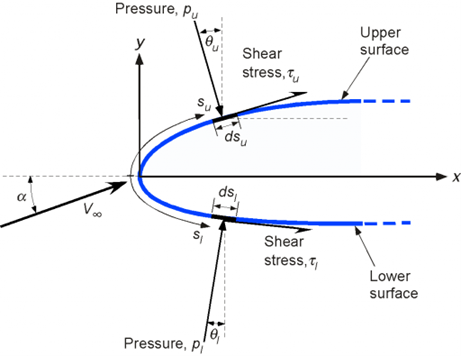
\includegraphics[width=\linewidth]{Images/ShearStress.png}
    \caption{Pressure and Shear Stress on an Aerodynamic Surface}
    \label{fig:pressure and shear}
\end{figure}
Since a force is a pressure multiplied by an area, $F=PA$, we can integrate our pressure distribution over an area to understand the total forces that are acting on a geometry. Often, we see this expressed in the form of an integral over the length of the geometry. This length is denoted $c$, the chord length, in the example of the airfoil. These integrals are shown below:
\begin{gather}
    N'=\int_0^{c}{p_lu-p_u}{dx}+\int_0^{c}{\left[\tau_u\frac{dy_u}{dx} + \tau_l\frac{dy_l}{dx}\right]}{dx}\\\\
    A'=\int_0^{c}{\left[p_u\frac{dy_u}{dx} + p_l\frac{dy_l}{dx}\right]}{dx}+\int_0^c{(\tau_u+\tau_l)}{dx}
\end{gather}
Where the $N'$ and $A'$ are the normal and axial force on the aerodynamic surface. Here, the apostrophe (We would say 'N prime') refers to the fact that the force acts over a unit length in the $\hat{z}$ direction. We are assuming a unit length here since we are considering the 2-D case in this example. More generally, we would perform this calculation more generally in 3D, but that is beyond the scope of this example.

The normal force acts normal in the $\hat{y}$ direction and the axial force acts in the $\hat {x}$ direction as shown in Figure \ref{fig:pressure and shear}. Normal and axial forces are not commonly used in our modeling outside of these calculations. More often, we see the quantities lift and drag, which are defined with respect to the freestream velocity. Using our knowledge from section \ref{sec:2D Rotations}, we can easily transform our normal and axial forces into a lift and drag using a rotation matrix with our angle of attack, $\alpha$. This rotation matrix takes the form:
\begin{equation}\label{eq:LDMatrix}
 \begin{bmatrix}
     D'\\L'
 \end{bmatrix}
 =\begin{bmatrix}
        cos\alpha &sin\alpha\\
        -sin\alpha&cos\alpha
    \end{bmatrix}
    \begin{bmatrix}
        A'\\N'
    \end{bmatrix}
\end{equation}
We can expand \eqref{eq:LDMatrix} to give two scalar equations:
\begin{gather}
        L'=N'cos\alpha-A'sin\alpha\\
        D'=A'cos\alpha+N'sin\alpha
\end{gather}
So, if we know the distribution of pressure over our body, we have shown that we can find the resultant aerodynamic forces acting on our body. As briefly described in Section \ref{sec:moments}, another important parameter to find is our center of pressure.
\subsection{Center of Pressure}
Simply stated, the center of pressure is the location at which all the aerodynamic forces acting on a body produce no resultant moment. This location is particularly useful for our case because we can assume that the lift and drag forces act through the center of pressure rather than assuming that lift and drag act as force distributions. This will make our future calculations much more simple, so we would like to know the center of pressure and how to calculate it.

To find the location where the center of pressure occurs, we can take the moment about any point first. Often, we choose to take the moment about the nose of the rocket (called the leading edge when referring to a wing), since we define the origin here. This integral has a similar form to the normal and axial force integrals, except that we multiply the force by the distance from the nose. For more information on why this is done, refer to \cite{gundersen_understanding_2020}. Writing out this integral, we get:
\begin{gather}
    M_{LE}'=\int_0^c{p_u-p_l}{dx}+\int_0^c{\left(\tau_u\frac{dy_u}{dx}+\tau_l\frac{dy_l}{dx}\right)}{xdx}\\+\int_0^c{\left(p_u\frac{dy_u}{dx}+\tau_u\right)}{y_udx}+\int_0^c{\left(-p_l\frac{dy_l}{dx}+\tau_l\right)}{y_ldx}
\end{gather}
Knowing the normal force and the moment about the leading edge, we can find the center of pressure location as:
$$x_{cp}=\frac{-M_{LE}'}{N'}$$
We note that the convention for the moment about the nose is for a positive moment to denote a pitch up (this is why the negative sign is present). This is opposite the convention established by the \gls{rhr}. For all other moments used in our 6-DoF models, we use the standard \gls{rhr} convention for moments.

For more information on the derivation of the equations in this section, refer to Chapters 1 and 2 of \cite{anderson_fundamentals_2017}.

For a rocket, we generally consider the body to be \textit{axisymmetric} about the longitudinal axis, when the whole structure can be rotated about the axis which we define as $\hat{X}$. 

Because our rocket is axisymmetric, we assume that the center of pressure always lies along the longitudinal axis. Although this assumption is not necessarily true, as we will see later, the largest effects on the aerodynamic moments will occur from changes along the longitudinal direction rather than changes along the \textit{transverse plane. }We can think of this intuitively because of the center of pressure separated from the center of mass by more than the diameter of the rocket, so changes in this direction have a greater effect.
\section{Atmospheric Modeling}
The first hurdle to overcome when describing the aerodynamics of our system is to find values for our freestream quantities. We explore the calculation of $V_{\infty}$ in Section \ref{sec: Newtonian Dynamics}. The other parameters we need to calculate are $\rho_{\infty}$ and $a_{\infty}$. Luckily, the standard density and Mach number of the atmosphere on Earth is well defined. In MATLAB, we can find this density at any altitude with "atmosisa" as:

\begin{lstlisting}[style=Matlab-editor]
    [T, a, P, rho] = atmosisa(height);
\end{lstlisting}
This gives us a standard value of $\rho_{\infty}$ and $a_{\infty}$ to use. However, the value of can vary by up to 10\% depending on the weather conditions \cite{svickova_air_2020}. Similarly, the Mach number has a strong dependence on temperature $\left(M=\sqrt{\gamma RT}\right)$, so the free-stream Mach number may also be different by 10-20\% of standard values. 

All of this is to say that using "atmosisa" gives us a good baseline model of the atmosphere but is not the final say in atmospheric modeling. For now, we use "atmosisa" in our modeling because we can live with this variation in our model. However, it may be useful in the future to use other sources of atmospheric data that give location and time specific data.

\chapter{Numerical Integration Schemes}

\begin{chapquote}{Wolfgang Pauli}
    ''The best that most of us can hope to achieve in physics is simply to misunderstand at a deeper level.''
\end{chapquote}
For more information and derivations about the following section, refer to \cite{trench_31_2020}. This source includes some more information than included here and some useful examples.

\section{Euler Integration}
We have previously discussed the simplest integration scheme, the explicit Euler method, which we used in Section \ref{sec: Numerical Integration in the 1DoF}. Understanding the Euler method is key to understanding and using more complex integration schemes, so we recommend writing a few of your own Euler integration scripts in MATLAB or a coding language of your choice to really solidify your knowledge before moving on to more complex integration schemes. 

We formalize the explicit Euler integration below. Given a linear ODE:
$$y'=f\left(x,y\right)$$
With initial condition:
$$y(x_0)=y_0$$
We perform Euler integration first by defining an interval over which to perform the numerical integration. For Euler integration, we equally space these points by our timestep, $dt$. We can parameterize these points as:
$$x_i=x_0+i\Delta t$$
Our next step is to find the value of the tangent line at each point. This is trivial, since our differential equation tells us what $y'$ looks like at any value. All we have to do is evaluate:
$$y'=f\left(x_i,y(x_i)\right)$$
The problem here is that $y(x_i)$ is an unknown quantity (if we knew it, we wouldn’t have to do integration). So, to find the value of $y(x_i)$ we take an iterative approach. We know the starting value, $y(x_0)=y_0$, so we can find an approximation of the new value by multiplying the timestep by the current slope. For the first timestep this will look like:
$$y_1=y_0+\Delta t\cdot f(x_0,y_0)$$
Now that we’ve found an approximation for $y_1$, we can extend this to find approximations for $y_2$, $y_3$, and so on. This formula is generally extensible as:
$$y_{n+1}=y_i+\Delta t \cdot f(x_i,y_i)$$
We represent this Euler integration scheme graphically with a simple example. Suppose our differential equation is $y'=2x$ with initial condition $y(0)=0$. In this example, we can see from inspection that the solution curve is $y=x^2$. Performing Euler integration with a $\Delta t$ of 0.5 yields the black approximation in Figure \ref{fig:Euler}.


\begin{figure}[ht]
    \centering
    
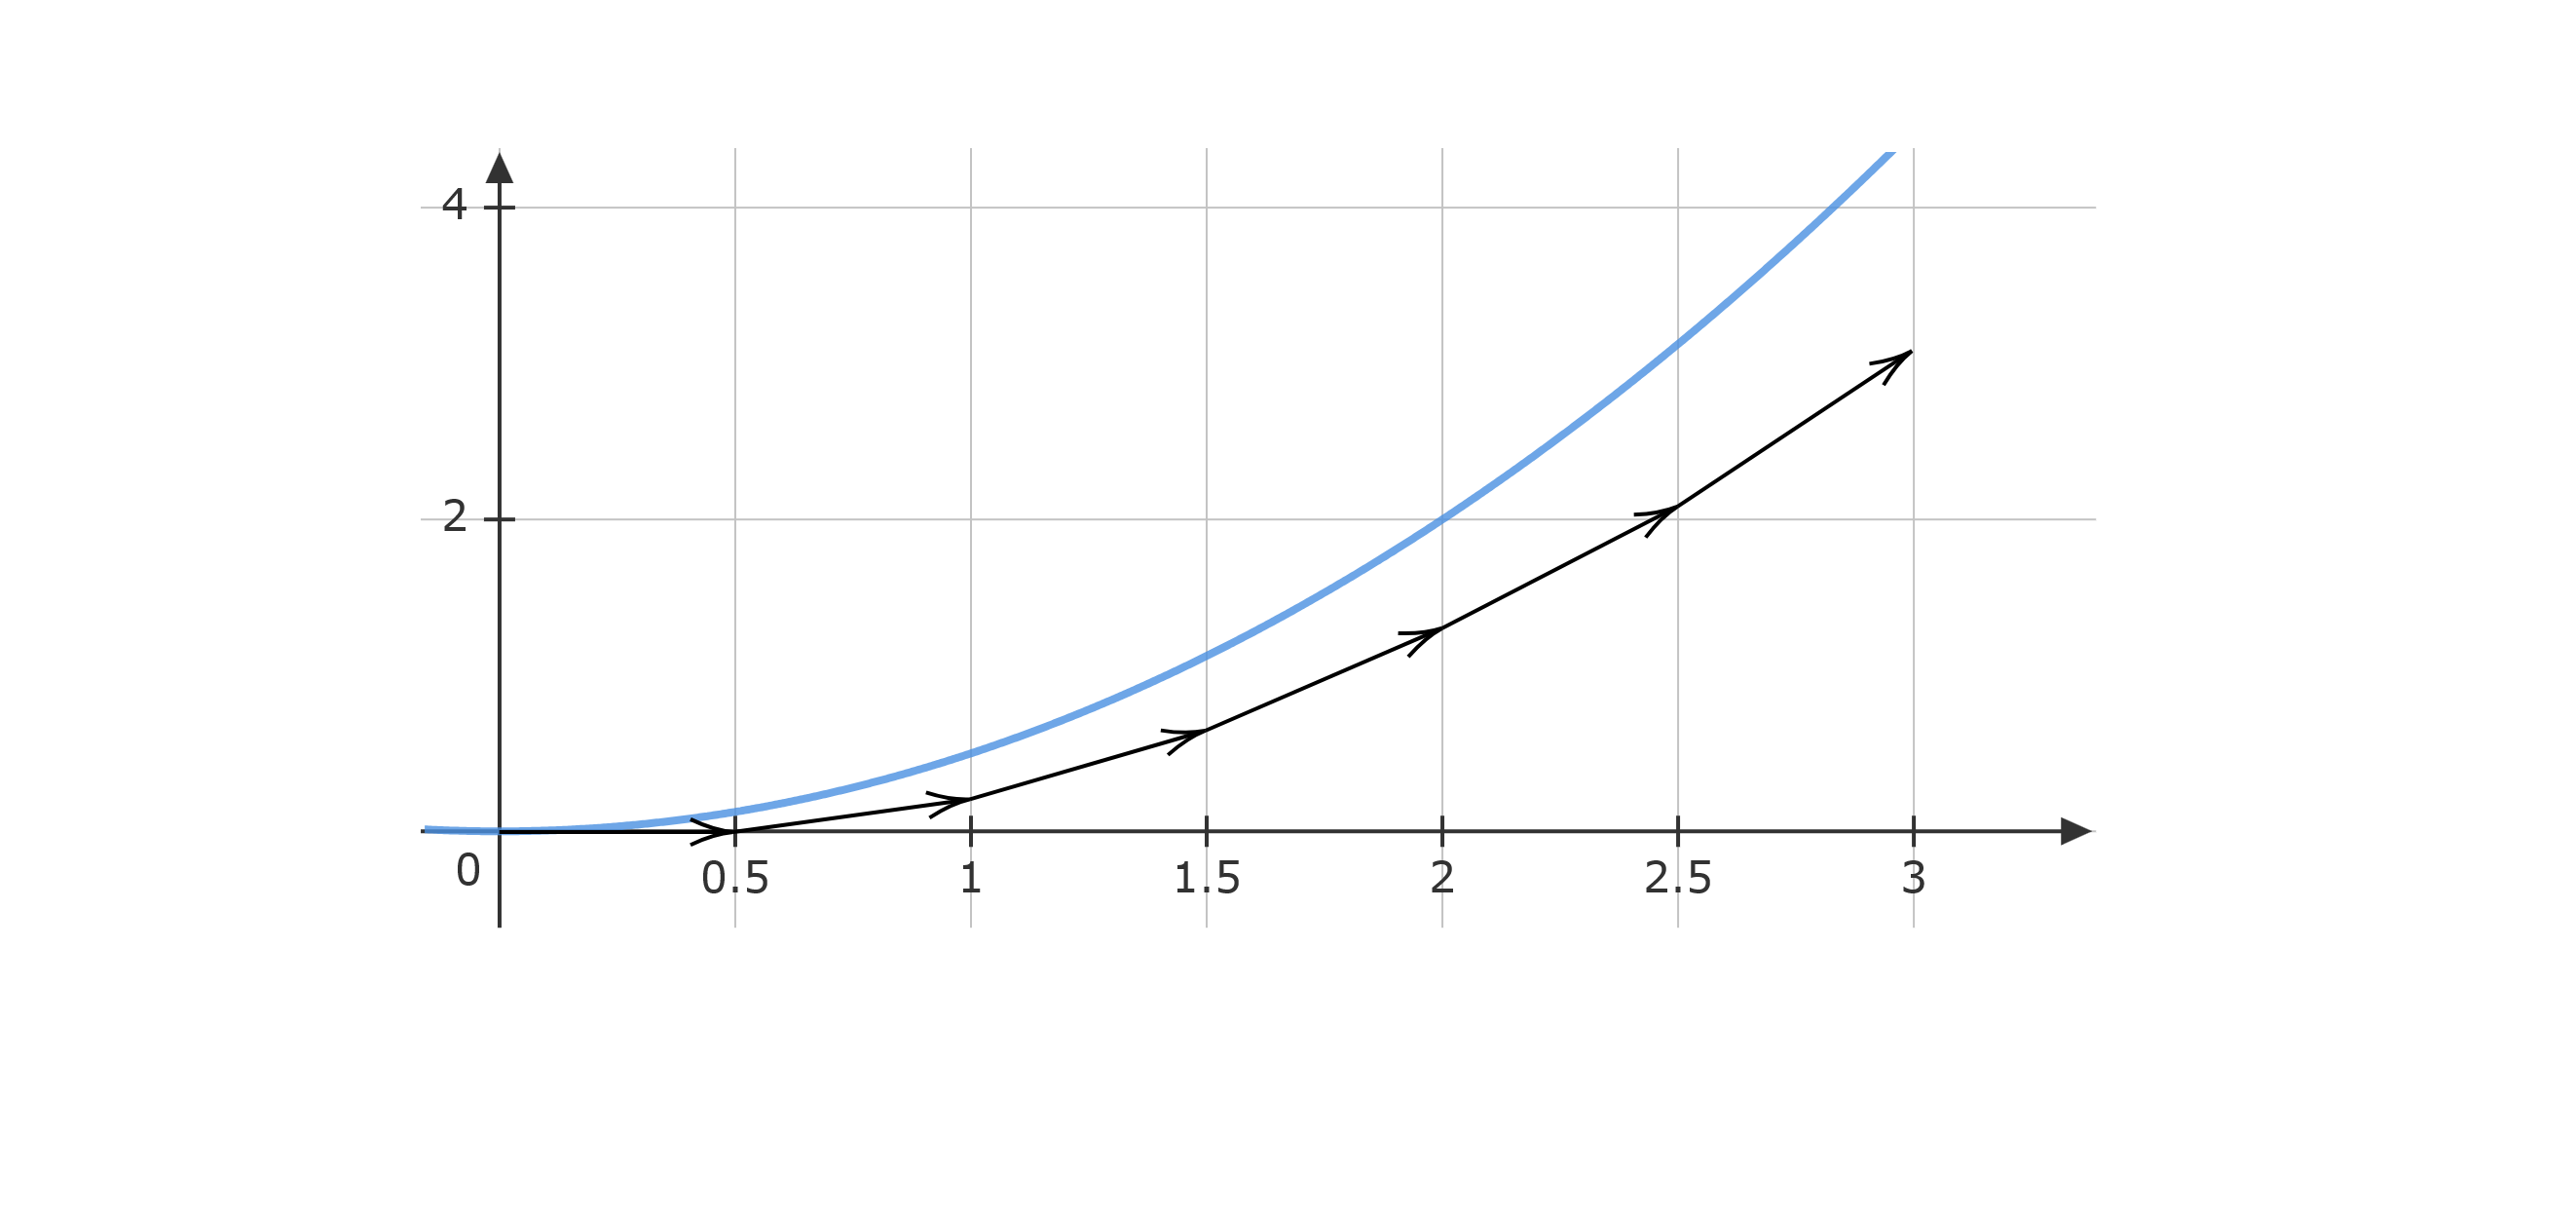
\includegraphics[width=\linewidth]{Euler.png}
    \caption{Euler Method Numerical Approximation}
    \label{fig:Euler}
\end{figure}

As can be seen from the \ref{fig:Euler}, large timesteps quickly lead to error in the solution. For a strictly convex curve, our Euler approximation will always give us an under-approximation of the solution. In some cases, however, our solution may diverge so greatly that it becomes unstable and values tend toward infinity.\footnote{This is especially true for periodic functions. When working with periodic functions, make sure to sample well below the Nyquist limit.}

In Table 2 below, we describe the benefits and drawbacks of Euler integration.

%% add stupid table here

\subsection{Errors in the Euler Method}
We will use the example of the Euler Method to demonstrate error in numerical integrators. These same concepts will apply when we move on to higher order integrators. 

Errors in the integration scheme come from two different sources:

1. Euler integration schemes only account for linear terms because it only considers the slope of the tangent line at a point. Thus, any quadratic order terms or higher will not be accounted for. Thus, the error is proportional to the timestep squared, $\Delta t^2$.\footnote{This intuitive explanation is not entirely correct, see (3) for a full derivation using the Taylor Series. We also note that the technically correct way to denote this is $O(\Delta t^2)$, meaning the error is of order $\Delta t^2$} We call this error \textit{truncation error.}

2. Another problem is the fact that computers don’t have infinite precision. The loss of precision during computing is called \textit{roundoff error.}

It is worth noting that these errors are per timestep! So over the course of a full simulation, our errors will grow much larger than the error bounds that we’ve calculated above. In fact, for the Euler Method described above, the global error is proportional to the timestep, $\Delta t$.

We can of course, reduce errors in the simulation by reducing our timestep, $\Delta t$. However, this will also increase the computation time. Additionally, doing so will not reduce the roundoff error in the simulation. With more calculations being done, the roundoff error will have a larger impact. Thus, it is worthwhile to investigate other integration schemes.

\section{Improved Euler / RK2}
Given the limitations of the Explicit Euler method, we will start by investigating the improved Euler Method. This improved Euler method is the first of a family of integration schemes known as Runge-Kutta (RK) integration schemes. The number, 2, represents the order of the integration scheme, which we will explore more later.

The main area that led to inaccuracies in the explicit Euler method was the slope that we calculated. We can improve on this by taking two points and finding the average slope. We choose to take a point at our start and our end point,  and , and evaluate the slope at both of those points and average them. From the previous section, we can remember that:
\begin{equation}
    y'=f\left(x_i,y(x_i)\right)
\end{equation}
So, we can write the average slope as
\begin{equation}
    m=\frac{y_1'+y_2'}{2}
\end{equation}
Where
\begin{gather}
    y_1'=f\left(x_i,y(x_i)\right)\\
    y_2'=f\left(x_{i+1},y(x_{i+1})\right)
\end{gather}
Now that we have the slope, we follow the same process as we did for the Explicit Euler method to find the next value. We take the slope and multiply it by the timestep, $\Delta t$, and add the current value, $y(x_i)$. This gives us our approximation as:
\begin{equation}
    y=y(x_i)+\frac{y_1'+y_2'}{2}\Delta t
\end{equation}
We can write this then as:
\begin{equation}
    y_{i+1}=y_i+\frac{\Delta t}{2}\left[f(x_i,y(x_i))+f(x_{i+1},y(x_{i+1}))\right]
\end{equation}
To rewrite this equation in a way that is better suited for code:
\begin{gather}\label{eq:rk2}
    y_{i+1}=y_i+\frac{\Delta t}{2}(k_1+k_2)\\\\
    k_1=f(x_i,y_i)\\
    k_2=f(x+\Delta t, y_i+\Delta tk_1)
\end{gather}
We can note here that this method requires at least two evaluations since $k_2$ is dependent on $k_1$. However, this is often still more computationally efficient than the Explicit Euler method because larger time steps can be used with lesser error.

\subsection{RK2 in Code}
Implementing the RK2 algorithm in code is slightly more complicated than implementing the explicit Euler method. To properly implement this, we will use \textit{function handles} in MATLAB. Function handles act as pointers to an instance of a function. To explain what that means, we will examine the following code snippet:
\begin{lstlisting}[style=Matlab-editor]
f = @computeSquare;
a = 4;
b = f(a)
\end{lstlisting}
where "computeSquare" is defined as:
\lstset{style=mystyle}
\begin{lstlisting}[style=Matlab-editor]
function y = computeSquare(x)
y = x.^2;
end
\end{lstlisting}

The function handle allows us to assign the function to a variable, which we are calling "f". We call this a pointer because this variable ‘points’ to the function "computeSquare".

In this example, when we call this operation, we get "b=16" in the command window. The power of this is that we could instead pass in a vector of values for "a" and get outputs from the function for all of them. If we instead input:
\begin{lstlisting}[style=Matlab-editor]
f = @computeSquare;
a = [4,6,10];
b = f(a)
\end{lstlisting}
We get an output of "b = 16  36  100". The usefulness of this is immediately apparent for numerical integration. We can pass in a vector of many different times and get outputs for each of them. 

Another useful feature of function handles for numerical integration is that they allow us to pass in only the variables needed for numerical integration and pass other variables in the expression as constants. In general, we want our numerical scheme to only accept our state vector and the time vector. This is the same thing that "ode45" does, so it is best practice to do the same thing here.

%% more on the code needed here

\section{RK4 Integration}
RK4 integration is the last major integration scheme that we will explore. RK4 integration is often the best balance between the precision of the algorithm and the speed of computation. 

To explain the RK4, we will go back to the RK2 and explain it in a slightly different way that will shed light on what we are doing with RK4. In RK2, we described taking the average slope of the function. We can also imagine taking the Taylor expansion of our function:
$$y_{i+1}=y_i+y_i'\Delta t+y_i''\frac{\Delta t}{2}+O\left(\Delta t^3\right)$$
From this Taylor expansion of the solution, we can that our approximation accounts for linear and quadratic terms. Thus, our error is proportional to terms to the 3\textsuperscript{rd} power, represented by $O(\Delta t^3)$. We know  and , but the 2\textsuperscript{nd }order derivative of our function is unknown. We can approximate this 2\textsuperscript{nd} order derivative as:
$$y_i=\frac{y'_{i+1}-y_i'}{\Delta t}$$
Upon rearranging this equation, we can see that we arrive at the same expression as we did before. We can apply the same approach for the RK4 integration, except we consider terms up to the 4\textsuperscript{th} order expansion of the Taylor series:
$$y_{i+1}=y_i+y_i'\Delta t+y_i''\frac{\Delta t}{2}+y_i'''\frac{\Delta t}{6}+y_i''''\frac{\Delta t}{24}O\left(\Delta t^5\right)$$
Immediately, we can see that our error has shrunk to be proportional to terms of the 5\textsuperscript{th} order, a dramatic reduction as compared to RK2 or Explicit Euler method.

\subsection{RK4 Integration in Code}
The RK4 Integration scheme can be expressed as a set of equations very similar to what we did with \eqref{eq:rk2}. We will not derive these equations here, because the process is very similar to that used for the RK2 method.

The form of these equations is shown in \eqref{eq:RK4}.
\begin{gather}\label{eq:RK4}
    y_{i+1}=y_i+\frac{\Delta t}{6}\left(k_1+2k_2+2k_3+k_4\right)\\\\
    k_1=f(x_i,y_i)\\
    k_2=\left(x_i+\frac{\Delta t}{2},y_i+\frac{\Delta t}{2}k_1\right)\\
    k_3=\left(x_i+\frac{\Delta t}{2},y_i+\frac{\Delta t}{2}k_2\right)\\
    k_4=f(x_i+\Delta t,y_i+\Delta tk_3)
\end{gather}
An implementation of this algorithm into code is shown below.
\begin{lstlisting}[style=Matlab-editor]
%% RK4 Integrator
% numerically integrates a first order initial value problem
% inputs:
% fun - function of integration
% dt - time step [s]
% tIn - input time [s]
% xIn - initial value input vector
% outputs:
% out - final value output vector
function out = rk4(fun, dt, tIn, xIn)
    f1 = fun(tIn,xIn);
    f2 = fun(tIn + dt/2, xIn + (dt/2) .* f1);
    f3 = fun(tIn + dt/2, xIn + (dt/2) .* f2);
    f4 = fun(tIn + dt, xIn + dt*f3);
    
    out = xIn + (dt / 6)*(f1 + 2*f2 + 2*f3+f4);
end
\end{lstlisting}
Often, we use a function in MATLAB called "ode45" to perform RK4 integration. This function has the benefit that it will change the step size to produce high accuracy when needed and decrease computation time otherwise.

An understanding of the operation of "ode45" is best motivated by an example. We include an example of a Lorenz Attractor in the Appendix \ref{sec:Lorenz Attractor RK4 Example} as an example of ode45. We recommend reading through this code and running it, as well as changing parameters to see how it affects the outputs.
\section{Other Integration Schemes}

\section{Code Optimization with Numerical Integration}
\subsection{Monte Carlo Simulation}
Often, we want to run many simulations with various parameters to gain a better understanding of our system. We call this method of running many simulations the \textit{Monte Carlo} method. Using the Monte Carlo method, we can ascertain information about the likelihood of certain events or approximate quantities that are hard to find analytically by running a large number of simulations and performing statistical analysis on the results. In this document, we will not dive into the methods of statistical analysis and the best ways to perform Monte Carlo simulations. This topic is very deep and is the focus of many peoples’ whole careers.

However, even with only rudimentary analysis, Monte Carlo can prove very useful. We will use the example of Monte Carlo to motivate the need for fast simulations. Often, we run upwards of 1000 simulations and fast computation is necessary to perform this large number of simulations. In this section, we will dive into the various methods to optimize MATLAB code and best practices for flight dynamics.
\subsection{Array and Function Optimizations}
MATLAB is generally quite computationally efficient at computing arrays and matrices. After all, MATLAB is ‘MATrix LABoratory’. However, we still need to be mindful of optimizations to our code.

It is best practice to only import what you need for a function or subroutine. For example, if you have wind data for all of the months out of the year, it is desirable to cull that down to the specific month before running the simulation.

Additionally, it is also beneficial for any imported data or long matrices to be passed into a function rather than called inside a function. \textbf{This is especially important inside the numerical integration scheme! }Running readmatrix inside of ode45 or whichever other numerical integration scheme you are using can slow down code upwards of 500\% depending on the length of the matrices being read.

Instead, it is best to pass these arrays into the function. Performing readmatrix can be slow because it must check if the values are numeric and organize them into tables. By passing only MATLAB arrays, computations are much faster.
\subsection{Flame Graphs for Optimization}
One important method of optimization is the MATLAB profiler. The primary capability of the profiler is the flame graph. An example of the flame graph is shown below in Figure 15.

The flame graph gives a visual representation of how long the code spends on each function. Functions in blue are those defined by the user. Those in grey are built in MATLAB functions.

%% Figure here
Poorly optimized code will spend a long time running an excessive number of operations. In some cases, this is unavoidable. For example, ode45, which runs the RK4 integration scheme we discussed in section 5.3, must run for every time step and is likely to comprise a large part of simulation time.

However, other operations, such as "atmosisa", should not comprise a large portion of simulation time. As seen in Figure 15, calling the atmosisa function on every loop takes about 40\% of the total time spent in ‘RK4Integrator’ function. By instead creating a table of the atmosisa data before running the simulation, we can reduce the runtime quite drastically. Implementing this simple change, we can see the reduction in simulation time as shown in Figure 16.

% figure here


\chapter{The 6-DoF}

\chapter{Appendix}
\section{Code}
This section contains lengthier segments of example code from either the 6-DoF itself or a proof/example relating to it. Refer to the section numbers to find the appropriate implementation of each code segment.
\subsection{Lorenz Attractor RK4 Example}\label{sec:Lorenz Attractor RK4 Example}
\lstinputlisting[style=Matlab-editor, caption = Lorenz Attractor]{LorenzAttractor.m}\label{code:Lorenz}

We also have a script to display the results of this in a nice animation:

\lstinputlisting[style=Matlab-editor, caption =Lorenz Animation]{LorenzAnimation.m}\label{code:LorenzAnim}

\printglossary

\printbibliography[heading=bibintoc, title={References}]

\end{document}
